\documentclass[twoside,a4,12p]{report} %,draft,openright]

\usepackage{epsf,graphicx}
\usepackage{latexsym,amssymb}
\usepackage{setspace,cite}
\usepackage{array}
\usepackage{amsmath}
\usepackage{fancyhdr}
\usepackage{float}
\usepackage[LGRgreek]{mathastext}
\usepackage{lipsum}
\usepackage{multirow}
\usepackage{subfigure}
\usepackage{url}
\usepackage{varwidth}
\usepackage{booktabs}
\usepackage[table]{xcolor}
\usepackage{tabularx}
\usepackage{arydshln}
\usepackage{datatool}
\usepackage{courier}
\usepackage{lscape}
\usepackage{pdflscape}
\usepackage{siunitx}
\usepackage{bbding}
\usepackage{pifont}
\usepackage{wasysym}
\usepackage{amssymb}
% for margins left, right top bottom
\usepackage{anysize}
\marginsize{4cm}{2.5cm}{4cm}{4cm}

%\usepackage{draft} %draft option - doesn't put full figures in -
            % useful when editing

%does the headers on the pages - keep in
\usepackage{fancyhdr}


%omitting any of these makes the thesis compile without the omitted
%chapter - good for editing single chapters.
\includeonly{header,intro,background,appendix}
\usepackage{acro}
\DeclareAcronym{cad}{
  short = CAD,
  long  = Computer Aided Diagnosis
}

\DeclareAcronym{gt}{
  short = GT,
  long  = Ground Truth
}

\DeclareAcronym{acr}{
  short = ACR,
  long  = American College of Radiology
}

\DeclareAcronym{fa}{
  short = FA,
  long  = Fibro-Adenoma
}

\DeclareAcronym{dic}{
  short = DIC,
  long  = Ductal Inflating Carcinoma
}

\DeclareAcronym{ilc}{
  short = ILC,
  long  = Inflating Lobular Carcinoma
}

\DeclareAcronym{dr}{
  short = DR,
  long  = Diabetic Retinopathy
}

\DeclareAcronym{dme}{
  short = DME,
  long  = Diabetic Macular Edema
}

\DeclareAcronym{oct}{
  short = OCT,
  long  = Optical Coherence Tomography
}

\DeclareAcronym{sdoct}{
  short = SD-OCT,
  long  = Spectral Domain OCT
}

\DeclareAcronym{amd}{
  short = AMD,
  long = Age-related Macular Degeneration
}

\DeclareAcronym{pca}{
  short = PCA,
  long = Principal Component Analysis
}

\DeclareAcronym{nlm}{
  short = NLM,
  long = Non-Local Means
}

\DeclareAcronym{who}{
  short = WHO,
  long = World Health Organization
}

\DeclareAcronym{ncd}{
  short = NCD,
  long = Non-Communicating Diseases
}

\DeclareAcronym{ria}{
  short = RIA,
  long = Retinopathy Image Analysis
}

\DeclareAcronym{bm3d}{
  short = BM3D,
  long = Block Matching 3D filtering
}

\DeclareAcronym{snr}{
  short = SNR,
  long = Signal-to-Noise Ratio
}

\DeclareAcronym{psnr}{
  short = PSNR,
  long = Peak Signal-to-Noise Ratio
}

\DeclareAcronym{ssdc}{
  short = SSDC,
  long = Subspace-based Spatial Domain Constraint
}

\DeclareAcronym{dct}{
  short = DCT,
  long = Discrete Cosine Transform
}

\DeclareAcronym{obnlm}{
  short = OB-NLM,
  long = Optimized Bayesian NLM
}

\DeclareAcronym{pgpd}{
  short = PGPD,
  long = Patch Group Based nonlocal self-similarity prior learning for image Denoising
}

\DeclareAcronym{gmm}{
  short = GMM,
  long = Gaussian Mixture Models
}

\DeclareAcronym{db}{
  short = $dB$,
  long = decibels
}
\DeclareAcronym{svm}{
    short = SVM, 
    long = Support Vector Machine
}
\DeclareAcronym{bow}{
    short = BoW, 
    long = Bag of Words
}
\DeclareAcronym{rf}{
    short = RF, 
    long = Random Forest
}
\DeclareAcronym{auc}{
    short = AUC, 
    long = Area Under the Curve
}
\DeclareAcronym{rbf}{
    short = RBF, 
    long = Radial Basis Function
}
\DeclareAcronym{lbp}{
    short = LBP, 
    long = Local Binary Pattern
}
\DeclareAcronym{lbptop}{
    short = LBP-TOP,
    long = Three Orthogonal Planes
}
\DeclareAcronym{hog}{
    short = HoG, 
    long = Histogram of Oriented Gradients
}
\DeclareAcronym{se}{
    short = SE, 
    long = sensitivity
}
\DeclareAcronym{sp}{
    short = SP, 
    long = specificity
}
\DeclareAcronym{acc}{
    short = ACC, 
    long = accuracy
}
\DeclareAcronym{pre}{
    short = PRE, 
    long = precision
}
\DeclareAcronym{f1s}{
    short = F1-s, 
    long = F1-score
}
\DeclareAcronym{ltpocv}{
    short = LTPO-CV, 
    long = leave-two-patients-out cross-validation
}
\DeclareAcronym{seri}{
    short = SERI, 
    long = Singapore Eye Research Institute
}
\begin{document}
\newpage

%Puts page numbering of preamble in roman and of main body of thesis in
%arabic. Also defines how chapters and sections are made
\pagenumbering{arabic}
\setcounter{page}{1} \pagestyle{fancy}
\renewcommand{\chaptermark}[1]{\markboth{\chaptername%
\ \thechapter:\,\ #1}{}}
\renewcommand{\sectionmark}[1]{\markright{\thesection\,\ #1}}

%DEFINES TITLE PAGE, and contains abstract, acknowledgements, etc.

%%%%%%%%%%%%%%%%%%%%%%%%%%%%%%%%%%%%%%%%%%%%%%%%%%%%%%%%%%%%%%%%%%%%%%%%%%%
% This is a sample header for a sample dissertation. Fill in the name,
% and the other information. LaTeX will work out the table of
% content, the list of figures and of tables for you.
%%%%%%%%%%%%%%%%%%%%%%%%%%%%%%%%%%%%%%%%%%%%%%%%%%%%%%%%%%%%%%%%%%%%%%%%%%%


\newpage
\thispagestyle{empty}

% ******* Title page *******
% **************************

\vspace*{2cm}
\begin{center}
{\Large\bf Automatic Classification And Segmentation Of OCT Images\\} \vspace{2cm} {\large
Khaled Abdulhameed Manea Alsaih\'i\\
\vspace{2cm}
Department of LE2I - Laboratoire Electronique, Informatique et Image \\
Université Bourgogne Franche-Comté \\
University of Technology Malaysia }
\end{center}

\vspace{7cm}
\begin{center}
{\large A Thesis Submitted for the Degree of \\MSc
in Vision and Robotics (MSCV) \\\vspace{0.3cm} $\cdot$ 2016
$\cdot$}
\end{center}
\singlespacing


%ABSTRACT
\begin{abstract}
We study in this thesis new methods in order to analyse Optical Coherence Tomography (OCT) volumes in patients that they suffer from Diabetes.
Early detection of Diabetic Macular Edema (DME) and Age-related Macular Degeneration (AMD) would help patients to get special treatments.
Thus, developing a mechanism or algorithm to automatically detecting the cyst is a must to save humans lives and maintain their status healthy. 

Basically, the algorithm for automated detection of the retina diseases is going through several steps.
Starting by preprocessing, which involves de-noising then flattening then cropping each B-scan of OCT images. After that, Multi-scale histograms of oriented gradient descriptors (HOG) and Local Binary Pattern (LBP) are extracted separately.
In other tests, HOG and LBP are combined to create a set of different feature vectors.
We also made some tests of the features vectors when projected into a lower-dimensional space through Principal Component Analysis (PCA).
Eventually, a Bag of Words (BoW) is also perform prior to feed the data to different classifiers like Linear SVM, kernel RBF SVM and Random Forest (RF).
Experimental results show a promising performance in terms of sensitivity (SE) and specificity (SP) of 87.5\% and 87.5\%, respectively, on a challenging dataset.
%$\lambda = \phi$ \ref{eq:eq1}
%\cite{}


\vspace*{5cm}



%\begin{center}
%\begin{quote}
%\it Research is what I'm doing when I don't know what I'm
%doing.\,\ldots
%\end{quote}
%\end{center}
%\hfill{\small Werner von Braun}

\end{abstract}

\doublespacing

%\pagestyle{empty}
\pagenumbering{roman}
\setcounter{page}{1} \pagestyle{plain}


\tableofcontents

\listoffigures
\listoftables

\chapter*{Acknowledgments}
\addcontentsline{toc}{chapter}
         {\protect\numberline{Acknowledgments\hspace{-96pt}}}

First of all, I would like to thank my amazing supervisor Prof. Fabrice Meriaudeau for his consistent support and clear directions. He never felt annoyed from my questions.
I would also love to thank my colleagues Glemaitre Lemaitre and Mojdeh Rastgoo for their kind help through the duration of my master project.

I would like to send this thesis work and efforts to My country YEMEN and then to my father Prof. Abdulhameed Alsaih and My Mom for their permanent support through my life.
Also I would like to thank my brother Tariq, my Sister Taif, my cousins Mojahed, Mohammed and Dr.Sakher. 

In addition, I would like to thank my friends that they Always support me starting by Hamodi, Yousef, Zezo, Sabahi, Seper, Paola, Jose, Dennis, Sandeep, Alhalali, Cansen, Raed, Kiril, and others.

As usual I would like to thank my Senior Dr.Fares, Dr.Taha and Dr.Abdulaziz for their motivation and help for any inquiries.   

Finally, thanks to University of Burgundy and University of Technology Malaysia for the great chance to be part of this course which taught me a lot and looking forward to apply it with the sense of serving humanity in a good manner.

\pagestyle{fancy}




\newpage

%sets up headers for lefthand and righthand pages. To alter, edit
%these lines and the chaptermark/sectionmark lines above
\addtolength{\headheight}{3pt} \fancyhead{}
\fancyhead[LE]{\sl\leftmark} \fancyhead[LO,RE]{\rm\thepage}
\fancyhead[RO]{\sl\rightmark} \fancyfoot[C,L,E]{}
\pagenumbering{arabic}

%\singlespacing
%\doublespacing
\onehalfspacing
\chapter{Introduction} \label{chap:intro}

%\section{Preparing your dissertation} \label{sect:thefirst}

%You are strongly encouraged to use the Latex templates provided.
Sugar level Discipline is what determine the existence of Diabetes in human body.
Diabetes has two types: type 1 which is insulin-dependent and type 2 which insulin-independent.
This critical disease is affecting many parts of the body like the Eye, Heart, Pancreas, body power and others.
The scope of this project is to focus in the Eye disease specifically Retina.
The sight for human is so important and with the Optical Coherence Tomography (OCT) images, the doctor can decide the status of the patient either it has disease or not.
Some statistics are showing from \cite{national1995diabetes} 29.1 million of Americans in the United States, which contributes to 9.3\% of the overall population.
Diabetes added to 231,404 deaths in the US in 2007.
\$245 billion is the total cost of diagnosing the disease in the United States in 2012.
With this big number of affected people and the money spent for Research and development (R\&D) in this area many algorithms are designed to detect diabetes in the early stage.

Eye diseases such as Diabetic Retinopathy (DR) and Diabetic Macular Edema (DME) are the most common causes of irreversible vision loss in individuals with diabetes.
DME is defined as the increase in retinal thickness within one disk diameter of the fovea center with or without hard exudate and sometimes associated with cysts.
Spectral Domain OCT (SD-OCT)\cite{cense2004ultrahigh} images the depth of the retina with a high resolution and fast image acquisition is an adequate tool, compared to fundus images for DME identification. Automated diagnosis on OCT imaging is rather new and most of the pioneer works on OCT image analysis have focused on the problem of retinal layers or specific lesions (e.g. cysts) segmentation. 

In this thesis we developed some methods to early detecting the diabetes with the care of some important things: time processing, cost and accuracy of the method in order to detect the cyst. We aimed to do many tests and use the tools provided to enhance the machine learning method we used.
The method applied is a great help for the doctors and for the patients if the solution of the sickness also involves any tele-medicine treatment. 

\section{Objectives} \label{sect:thefirst}
The project target is to develop an automatic algorithm for retina screening for the sake of detecting the cysts and during the research period the main objectives of this project as follows:

\begin{itemize}
\item \textbf{Objective 1}: develop an automatic algorithm to diagnose the retinopathy diabetes in the OCT volumes.

\item \textbf{Objective 2}: develop an automatic  algorithm to segment the cyst in OCT images using deep learning .

\item \textbf{Objective 3}: evaluate the algorithms based on diabetic retinopathy screening. 
\end{itemize}

After achieving the objectives, some other techniques was added to enhance the results.
In addition to the objectives mentioned, different classifiers was tested and compared.
An algorithm is developed to detect Diabetic Retinopathy (DR) and Diabetic Macular Edema (DME) from the lesions segmented.

\section{Thesis Overview}
This project is arranged and sequenced in four chapters. An outline is described as follows:

\begin{itemize}
\item \textbf{Chapter 2}: explains in details the anatomy of the eye accompanied by the diseases that affect the vision process for humans.
In addition, it reviews the previous work in this field with the state of art of this project.

\item \textbf{Chapter 3}: shows the work done in the period decided to do the project, which has two parts: first, designing an automatic algorithm to classify the OCT images.
Second, segmenting the OCT images based on deep learning techniques.

\item \textbf{Chapter 4}: Discusses the results of the work done and evaluate the performances of the methods.

\item \textbf{Chapter 5}: sums up the project and recommends work to be achieved in future.  
\end{itemize}

%\subsection{Paper}
%The manuscript should be in A4 size, and the printed paper should
%be of at least 70 gsm.
%
%\subsection{Font and margins}
%Thesis should be printed on both sides of the paper. Use no less
%than 1.5 spacing, with quotations and notes single-spaced.
%Regarding \textbf{Character size}, not less than 2.0mm for
%capitals and 1.5mm for x-height (the height of a lower-case x). Us
%a serif font (i.e. Times) between 10 and 12 points. Use consistent
%and clear fonts through all the document.
%
%The text layout should be approximately as follows:
%
%\begin{itemize}
%    \item $4cm$ binding margin
%    \item $2cm$ head margin (top of page)
%    \item $2.5cm$ fore-edge margin
%    \item $4cm$ tail margin (bottom of page)
%\end{itemize}

%\section{Title Page}
%The title page should contain the title of thesis, authors name,
%and at the foot of the page: the name of degree,  Your University,
%and the year of presentation. Something like this:
%
%\vspace*{1cm}
%\begin{center}
%{\Large\bf MSc. Thesis example VIBOT\\} \vspace{2cm} {\large
%Robert Mart\'i\\
%\vspace{1cm}
%Department of Computer Architecture and Technology\cite{platel1997plant} \\
%University of Girona}
%
%\end{center}
%
%\vspace{2cm}
%\begin{center}
%{\large A Thesis Submitted for the Degree of MSc Erasmus Mundus in
%Vision and Robotics (VIBOT)\\ \vspace{0.3cm} $\cdot$ 2008 $\cdot$}
%\end{center}
%
%
%\subsection{References}
%You can reference other authors by using the $cite command$
%\cite{Pokorski:1998hr}. You are encouraged to use bib files and
%let bibtex do the job for you.
\chapter{Background} \label{chap:background}

In this chapter the explanation is well-defined in term of the anatomy of the eye and the state of art for classification tasks.
This chapter explains the retina layers and the abnormalities that may accompany the eye during the human life to have a better understanding about the project scope and the reasons behind following the algorithm used.
After that, a review of previous work in classification of OCT images and the techniques to evaluate and compare the results of the method used.
Then, a short summary for the papers is reviewed, followed by making a highlight for the main references is presented for this project   

\section{Introduction}

\subsection{The Eye}

\begin{figure}[htb]
        \centering
        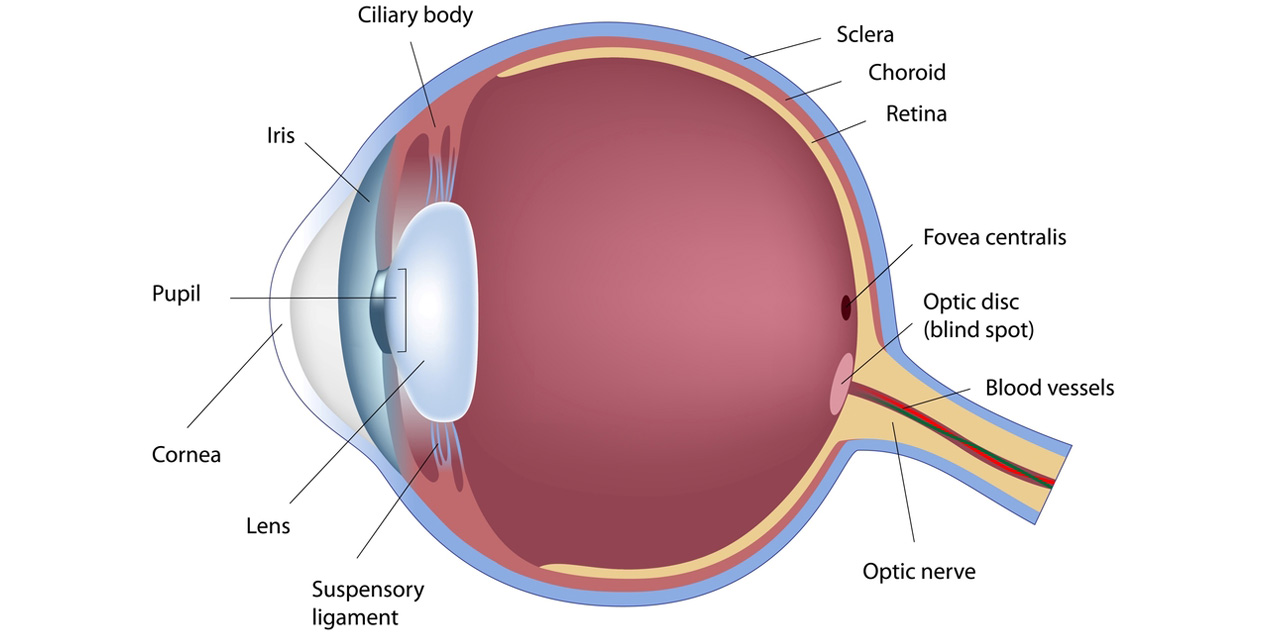
\includegraphics[width = 0.9\textwidth]{figures/Eye_anatomy.jpg} % scale, width, height 
  \caption{Anatomy of the Eye \cite{eyeimage}}
  \label{fig:Eyeanatomy}
\end{figure}  

Eye is one of the most important organs, which is responsible of vision for humans.
Saving this organ is critical and taking care of it is a must.
Many scientists have written the way the eye is working and they conclude, the eye is like a mirror so whatever it sees it reflects and in the very famous book (\textbf{Book of Optics}) \cite{alhazen1989book} written by Ibn Alhaytham, He claims "the eye is affected by light not the opposite".
In scientific view, the task of the eye is a sight machine that let the data received from the out atmosphere to be processed by brain for decision making for example: moving right ,left and etc... 
The camera idea was mainly gotten from the eye in the way it is working in term of light entrance to the lenses used then to the processor (Brain).
The camera creates pictures using films or digitally made \cite{abramoff2010retinal}.
Focus, contrast and the brightness also vary from camera to other based on how powerful the processor and other aspects.
The camera creates one image (Picture) or sequence of images (Video), it could be also in real time video like the eye with an advantage for the camera that it can record events for later use.
After observing how light travels by Ibn Alhaytham and his book he made the first pinhole camera to be the first design of camera and the development of the camera till our days.  
The anatomy of the eye is shown in Figure 2.1 with different layers, which is compromised with lenses to process data.
Humans may vary in the eye's structure, hence some people has a normal range of vision, others they can not see either far or near.
Eyes also can be infected by many diseases, which will be discussed after explaining the process of vision. 

Basically, the vision process can be explained as follows:
\begin{itemize}
\item \textbf{Cornea}: receives light for filtering.
Then, it focuses the data received.
\item \textbf{Aqueous Humour (Anterior Chamber)} : keeps the anterior part of the eye slightly curved and stable and it is made of viscous substance.
\item \textbf{Pupil}: adapts the eye lenses by relaxing or contracting depending on the amount of light enters the eye.
\item \textbf{Iris}: does the movement of the muscle based on the pupil order and based on the decision made by the pupil, the light will pass to retina
\item \textbf{Retina}: converts the light rays into electrical impulses to be delivered to the brain by optic nerve.

\end{itemize}
In our project we mainly focus in the retina part and it is explained as follows.

\subsubsection{Retina}
\begin{figure}[htb]
        \centering
        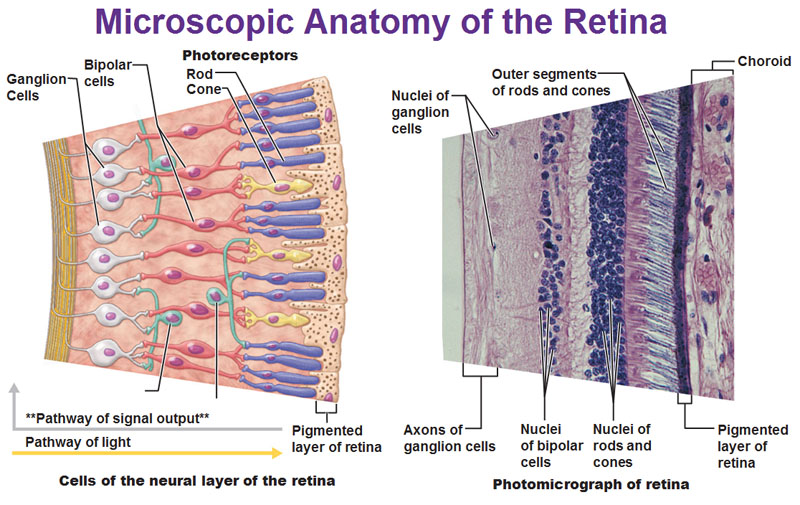
\includegraphics[width = 0.9\textwidth]{figures/Retina.jpg} % scale, width, height 
  \caption{Retina Anatomy \cite{retinaimage}}
  \label{fig:Retinaanatomy}
\end{figure}  
Retina is a multi-layered tissue located at the posterior of the eye.
Figure 2.2 shows the sensory parts in the retina, which they are the photo-receptors that get the rays and convert them into electrical impulses to be able to be read by the brain.
Impulses are passing through the optic nerve to the brain for image processing and the result of this process is the vision of the human.
There are millions of photo-receptors for sensing and there are two types of them based on their shapes : Rods and Cones.

Rods are located in periphery of the retina and they are imprecise and insensitive to colours so they can only recognize shapes in grey-scale.
Whenever there is a change in contrast it is very case-sensitive so it is most effective at night.
They are able to detect movement.    
Cones are responsible for day vision as they are very precise to detect colours.
They are located in the Macula \cite{mccaa1982eye}, \cite{abramoff2010retinal}.
The Fovea is the part of eye which is able to recognize the vision details. It is located in the central of the Macula.
Any accidental action to the eye results in losing Fovea will affect the vision in the central area.
A dense network of almost 1.2 million nerves is connecting the photo-receptors with the brain from the optic nerve.
The blind spot is located also in the retina, which has no photo-receptors.

The inner and outer layers of the retina  are encountered to be supplied by their fuel to enrich the retina with its need (oxygen and other important components required to keep the mechanism of vision) \cite{jonas1992count}.
The number of vessels for the inner layer 35\% is smaller compared to the outer layer 65\% to supply the retina.
Retina has many layers specified in \cite{abramoff2010retinal} as follows:
\begin{itemize}
\item Internal limiting membrane
\item Axons of the ganglion cells (Nerve Fibre Layer): the more the age, the thin it gets.
\item Ganglion Cell Layer includes the ganglion cells.
\item Inner Plexiform Layer have Amacrine and axons of bipolar cells.
\item Inner Nuclear Layer have horizontal and bipolar cells.
\item Outer Plexiform Layer includes horizontal dendrites and inner segments of photo-recepters cells.
\item The photo-receptors are located in the Outer Nuclear Layer.
\item External limiting membrane.
\item Finally, the layer that generates the colours to retina (Pigment Epithelium).
\end{itemize}
This complex combination of cells inside the retina is tremendous.
The existence of cysts is mysterious, thus it is studied by scholars to get the status of patients with different diseases \cite{jakobs2005retinal}

\subsection{Eyes Abnormalities}
Eyes abnormalities have no early signs, because the pain is not felt usually.
The vision also is not interrupted to give a warning that someone is infected by an eye disease to be diagnosed and get a treatment unless the problem is advance. 
As the body is a complex and compact system, hence any problem faces the eyes might interrupt many organs in the body and could be a sign to diagnose other diseases like heart diseases and diabetics.
The main disease, project making analysis on is the Diabetic Macular Edema (DME).

Diabetic sometimes called Diabetes mellitus (DM) where pancreas can not produce enough insulin or the cells can not respond to the insulin produced.
As of 2015, an estimated 415 million people have diabetes worldwide \cite{fernandez2010obesity}.
This represents 8.3\% of the adult population, with equal rates in both women and men \cite{vos2013years}.
The number of people with diabetes is expected to rise to 592 million by 2035 \cite{beagley2014global}.
The global economic cost of diabetes in 2014 was estimated to be \$612 billion USD \cite{atlas2013international}.
The best way to protect the eyes is by doing a regular visit to the doctor for eye examination.
Failing to treat this disease will yield to other diseases such as  cardiovascular disease, stroke, kidney failure and damage to the eyes.
In this section, many diseases that might hit the eye will be ordered alphabetically :
\begin{enumerate}
\item \textbf{Age-related Macular Degeneration (AMD)}: is a disease that will affect the Macula, which is located at the center of the retina.
Getting affected by AMD is a sign for diabetes.
AMD will lead to blur the vision, a dark area in the center of the vision and straight line distortion as shown in figure 2.3.
Activities required focus is affected by this disease like driving, cooking or studying.
There are two types of AMD: Dry and Wet. 
The wet AMD is happening due to generating new blood vessels in the Macula, which will lead to rapid lose of central vision.
In the other hand, dry AMD is happening due to the existance of drusen, which they are small yellow particles that they are deposited under the Macula.
Slowly, this particles will lead to lose the central vision and it is the most popular type \cite{bressler1988age}.
 
\begin{figure}[htb]
        \centering
        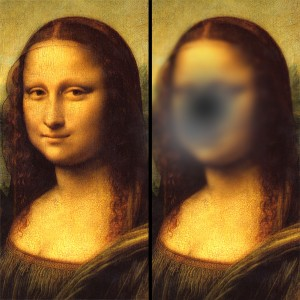
\includegraphics[width=0.45\textwidth]{figures/Centralloss.jpg} % scale, width, height 
  \caption{Loss of Central Vision \cite{centralloss}}
  \label{fig:Central Loss}
\end{figure}  
\item \textbf{Cataracts}: is an abnormality of the eye, which will affect the crystalline lens.
Crystalline lens is responsible in recognizing on stuff and people at different distances.
The typical effected patients in this syndrome is old people when the lens get stiffens due to ageing and they call it presbyopia.
In other ways, some people might face Cataracts earlier due to some reasons for example: diabetes, birth defects, steroids and heredity.
Cataracts patients will suffer from being sensitive to light, bad night vision, colour vision dimming, sometimes double vision in one eye and blurred vision \cite{klein1982cataracts}.
\begin{figure}[htb]
        \centering
        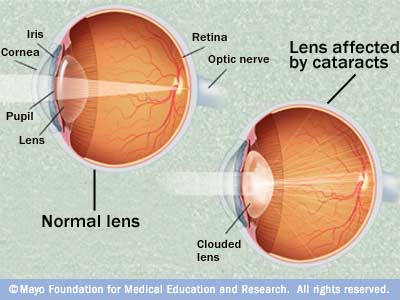
\includegraphics[width=0.7\textwidth]{figures/Cataracts.jpg} % scale, width, height 
  \caption{Cataracts \cite{cataracts2016}}
  \label{fig:Central Loss}
\end{figure} 
   
\item \textbf{Cytomegalovirus Retinis (CMV)}: is a disease that strikes the retina specifically the light sensing cells.
A quick treatment is required as this disease is so dangerous and sometimes might lead to blindness.
Cytomegalovirus Retinis does not produce symptoms and usually the immune system is able to fight it.
Sometimes, this virus will be accompanied by HIV virus.
This disease will make the patient suffer from couple of flashes for eyes, blind spots, end of the peripheral vision and blindness \cite{yeager1981prevention}.
\begin{figure}[htb]
        \centering
        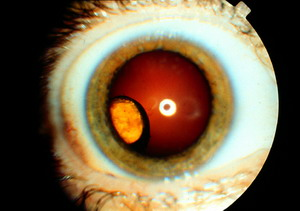
\includegraphics[width=0.3\textwidth]{figures/CMV.jpg} % scale, width, height 
  \caption{CMV and HIV \cite{CMV}}
  \label{fig:Central Loss}
\end{figure} 

\item \textbf{Diabetic Retinopathy (DR)} is disease that attacks the retina and it is a vascular complication.
Diabetic retinopathy (DR) is a vascular complication of DME that leads to vision loss in case of late treatment \cite{wilkinson2003proposed}.
Having Diabetes will increase the chances of getting blind than normal people.
\begin{figure}[htb]
        \centering
        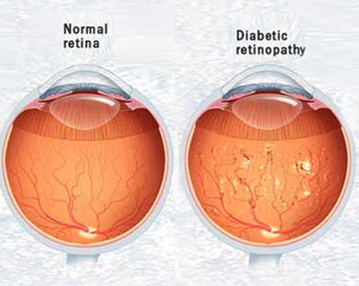
\includegraphics[width=0.6\textwidth]{figures/DR.jpg} % scale, width, height 
  \caption{Diabetic Retinopathy (DR) \cite{DR2016}}
  \label{fig:DR}
\end{figure}
\item \textbf{Diabetic Macular Edema (DME)} is a retinal disease and caused by fluid accumulation in the Macula dImaging of the eye is critical to improving the diagnosis, assessment of severity and progression, and evaluation of management of eye disease. 
It is also, a combination of complication of Diabetes Retinopathy that allows the fluid to escape.
The cones fill the Macula.
When the fluid starts to flow through the Macula to escape, blurred vision is the result of the inability of cones to sense the light.
Up to 30\% of Diabetes patients are suffering from DME. 
Two types of DME based on the way the fluid flow, which they are Focal DME and Diffuse DME.
To diagnose DME, retina thickness is checked if it is increased or exudate by 500 $um$ distance from the Macula centre \cite{bandello2010diabetic}.
DME only can be diagnosed by 3-D images because the lack of depth information when capturing the image due to the retina thickness increase.
Mainly, this project is focusing in detecting DME cysts and classifying the volumes based of how normal the volume is and DME shall look like the table in section 2.2.1

\item \textbf{Glaucoma}:this disease will damage the optic nerve, which is responsible for transferring data from the eye to the brain for image processing.
Thus, it will lead to vision loss or in the worst case scenario, blindness.
As other eye diseases, it is hard to diagnose the disease as it developed with no symptoms.
There are four types of Glaucoma: Chronic Open Angle Glaucoma, Acute Closed Angle Glaucoma, Secondary Glaucoma and Normal-Tension Glaucoma.
Glaucoma in case of acute angle will happen suddenly and the patient will vomit and feel dizzy. Also, it is accompanied with headache and vision blurring \cite{group1998comparison}.
\begin{figure}[htb]
        \centering
        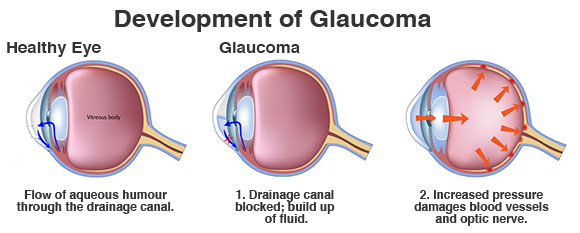
\includegraphics[width=0.75\textwidth]{figures/Glaucoma.jpg} % scale, width, height 
  \caption{Glaucoma \cite{Glaucoma}}
  \label{fig:Glaucoma}
\end{figure}

\item \textbf{Retinal Detachment}: a sudden damage of the retina allowing the fluid to flow inside it.
This action will make the retina to move away from the supportive tissue under it causing the detachment.
With this detachment, the retina is no longer able to correctly send the signals of light to the brain.
It can be treated but in a very good care \cite{retina1983classification}.
\begin{figure}[htb]
        \centering
        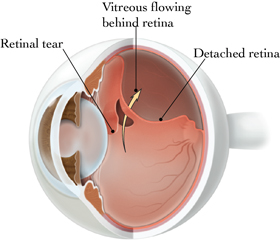
\includegraphics[width=0.5\textwidth]{figures/retinaldetachment.jpg} % scale, width, height 
  \caption{Retinal Detachment \cite{retinaldetachment}}
  \label{fig:Glaucoma}
\end{figure}
\end{enumerate}
 
\subsection{Imaging Techniques}
The eye imaging is critical in developing the diagnosing, analysing the progression and managing the evaluation of the disease.
The improvement in hardware such as chips and light sources and software such as image analysis is helpful in diagnosing the disease.
Based on the needed part of the eye and the disease to be imaged, the suitable imaging techniques are used by the ophthalmologists.
In this project, our data used are SERI and OPTIMA OCT images.
This section explains briefly ocular imaging techniques in the eye:

\begin{itemize}
\item \textbf{Scheimpflug principle}: this technique is named after its inventor the army captain Theodor Scheimpflug from Austria.
He has used it in creating a device for correcting the distortion in aerial photographs in a very systematic method.
This method has a rule that explains the orientation of the coordinates of optical system when the lenses are not in a parallel plane with the image plane.
It is can be used in corneal pachymetry, the corneal topography mapping, also prior to refractive eye surgery such as LASIK, and can be used in detection of keratoconus \cite{hockwin1987measuring}.
\begin{figure}[htb]
        \centering
        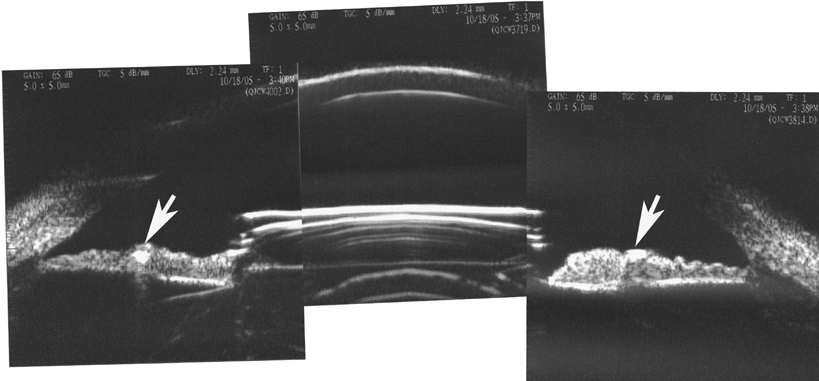
\includegraphics[width=0.7\textwidth]{figures/SPultra.jpg} % scale, width, height 
  \caption{Scheimpflug and ultrasonic \cite{SF2016}}
  \label{fig:Glaucoma}
\end{figure}

\item \textbf{Scanning laser ophthalmoscopy (SLO)}: this method is using confocal laser scanning microscopy for the aim of diagnosing the cornea and the retina at the eye of the human.
It employs scanning mirrors in horizontal and vertical coordinates for the aim of scanning a particular region in the retina and create a viewable images at the monitor.
It is also able to image the retina in real time and it might face a problem with reflections generated from the cornea.
It is helpful in term of diagnosing retinal disorders like DR, AMD, glaucoma and DME due to the high degree of spatial sensitivity \cite{gray2008vivo}.
It also has been developed to generate sharper images of the retina when it is combined with adaptive optics technology.
\begin{figure}[htb]
        \centering
        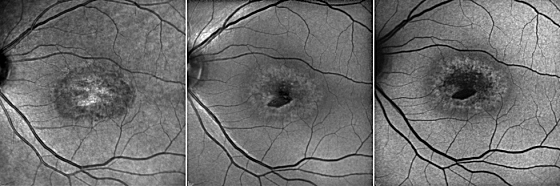
\includegraphics[width=0.6\textwidth]{figures/SLO.jpg} % scale, width, height 
  \caption{Scanning laser ophthalmoscopy \cite{SF2016}}
  \label{fig:Glaucoma}
\end{figure} 
\item \textbf{Ultrasonography}: this method uses mainly the time taken for high radio frequency pulses measurement, which is generated by piezoelectric devices.
The pulses is reflected by the interface of the ocular tissue(A-scan).
Another way of scanning (B-scan), which is inserting the probe across the eye to generate a section or moved in a rectangular pattern to create 3D form of structure \cite{cusumano1998three}.
As the emphasize of this method to use the high frequency pulses rather than light waves, it has the ability to penetrate opaque corneas to better image the ciliary body and surrounding parts.
Depth and resolution of ultrasonography penetration are affected by frequency's frequency.
\begin{figure}[htb]
        \centering
        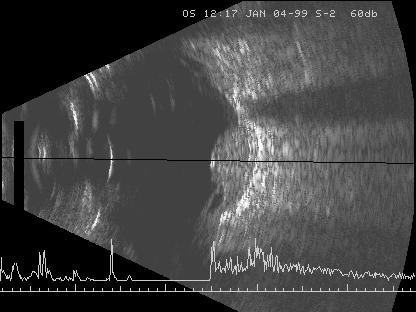
\includegraphics[width=0.4\textwidth]{figures/Ocularultra.jpg} % scale, width, height 
  \caption{Ocular Ultrasonography \cite{ocularultra}}
  \label{fig:Glaucoma}
\end{figure}
\item \textbf{Magnetic Resonance Imaging(MRI)}: is a well-known technique in imaging world, which results in producing a very detailed images of the internal frame of the body.
The principle of the MRI is based on nuclear magnetic resonance.
Spinning of the nuclei at certain radio frequency to obtain a stored signal that contains information about the the physical and chemical frame of molecules that has hydrogen.
Also, in the case of placing the object in an uniform magnetic field, the nuclear spins within the targeted structure.
Hence, they will align together wither in parallel or anti-parallel to the direction of the magnetic field flux.
Radio-frequency pluses will radiate echoes of the same frequencies which is detected.
The density of the nuclei and the internal structure will affect the magnitude and the decay of the signal.
Due to the high price of this device, so it has limited usage, but they use it in the ageing ciliary muscle diameter in phakic eyes \cite{strenk2004magnetic}, checking the 3D structure of the myopic, viewing gained ocular anomalies and some animal models in ocular drug-delivery systems\cite{kim2007assessment}.
\begin{figure}[htb]
        \centering
        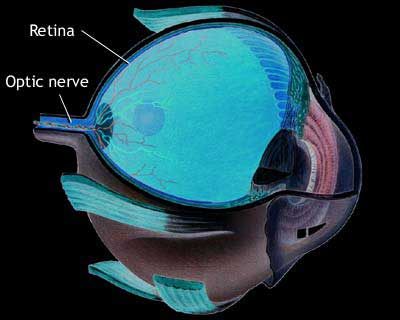
\includegraphics[width=0.3\textwidth]{figures/MRI.jpg} % scale, width, height 
  \caption{Magnetic Resonance Imaging \cite{MRI2016}}
  \label{fig:Glaucoma}
\end{figure}
\item \textbf{Optical Coherence Tomography (OCT)}: the main method of imaging in this project which is a light reflection based.
An interface is used instead of calculating the time between emission and detection of light-pulse owing to the fast speed of light in this technique, which is faster than sound speed in almost 872,000 times (344 $m/s$ speed of sound and OCT light speed is 299,792,458$m/s$).
Axial resolution is equal to light source coherence length and lateral resolution is the optics of the device function.
While, the laser (Conventional interferometry) has a long coherence length in meters, broadband of light sources are in use to make the laser frequencies shorten to micrometers in order to view high resolution eye image.
Any light outside the broadband of short frequencies length will not be used as data in the coherence pattern.
There are two types of OCT images, (A and B-scan).
A cross-sectional tomography (B-scan) is achieved by aligning a series of axial depths (A-scan).
(A-scan) is built by physically scanning the coherence length using the reference mirror in time domain OCT.
This type is limiting the resolution of the image and the images shall look like the table presented in section 2.2.1. 
(B-scan) is used to diagnose DME,AMD and Glaucoma with better precision than fundus images.    
\item \textbf{Optical Coherence Tomography Angiography (OCTA)} is another type of normal OCT, yet modern and from the name angiography, which means a technique to visualize the internal structure of organs and blood vessels.
OCTA uses motion contrast imaging to high-resolution volumetric blood flow data producing angiographic images in seconds.
OCTA matches the decorrelation signal (differences in the backscattered OCT signal intensity) between sequential OCT b-scans taken at accurately the same cross-section in order to create a map of blood flow.
Axial bulk motion from patient movement is removed so sites of motion between repeated OCT b-scans signify strictly erythrocyte movement in retinal blood vessels.
OCTA demands higher imaging speeds than most presently accessible OCT systems can deliver in order to attain a densely sampled volume.
Conventional OCT device scanning speeds would outcome in too much trade-off between reduced field of view, lower image quality, and greatly increased scanning time\cite{spaide2015retinal}.
\begin{figure}[htb]
        \centering
        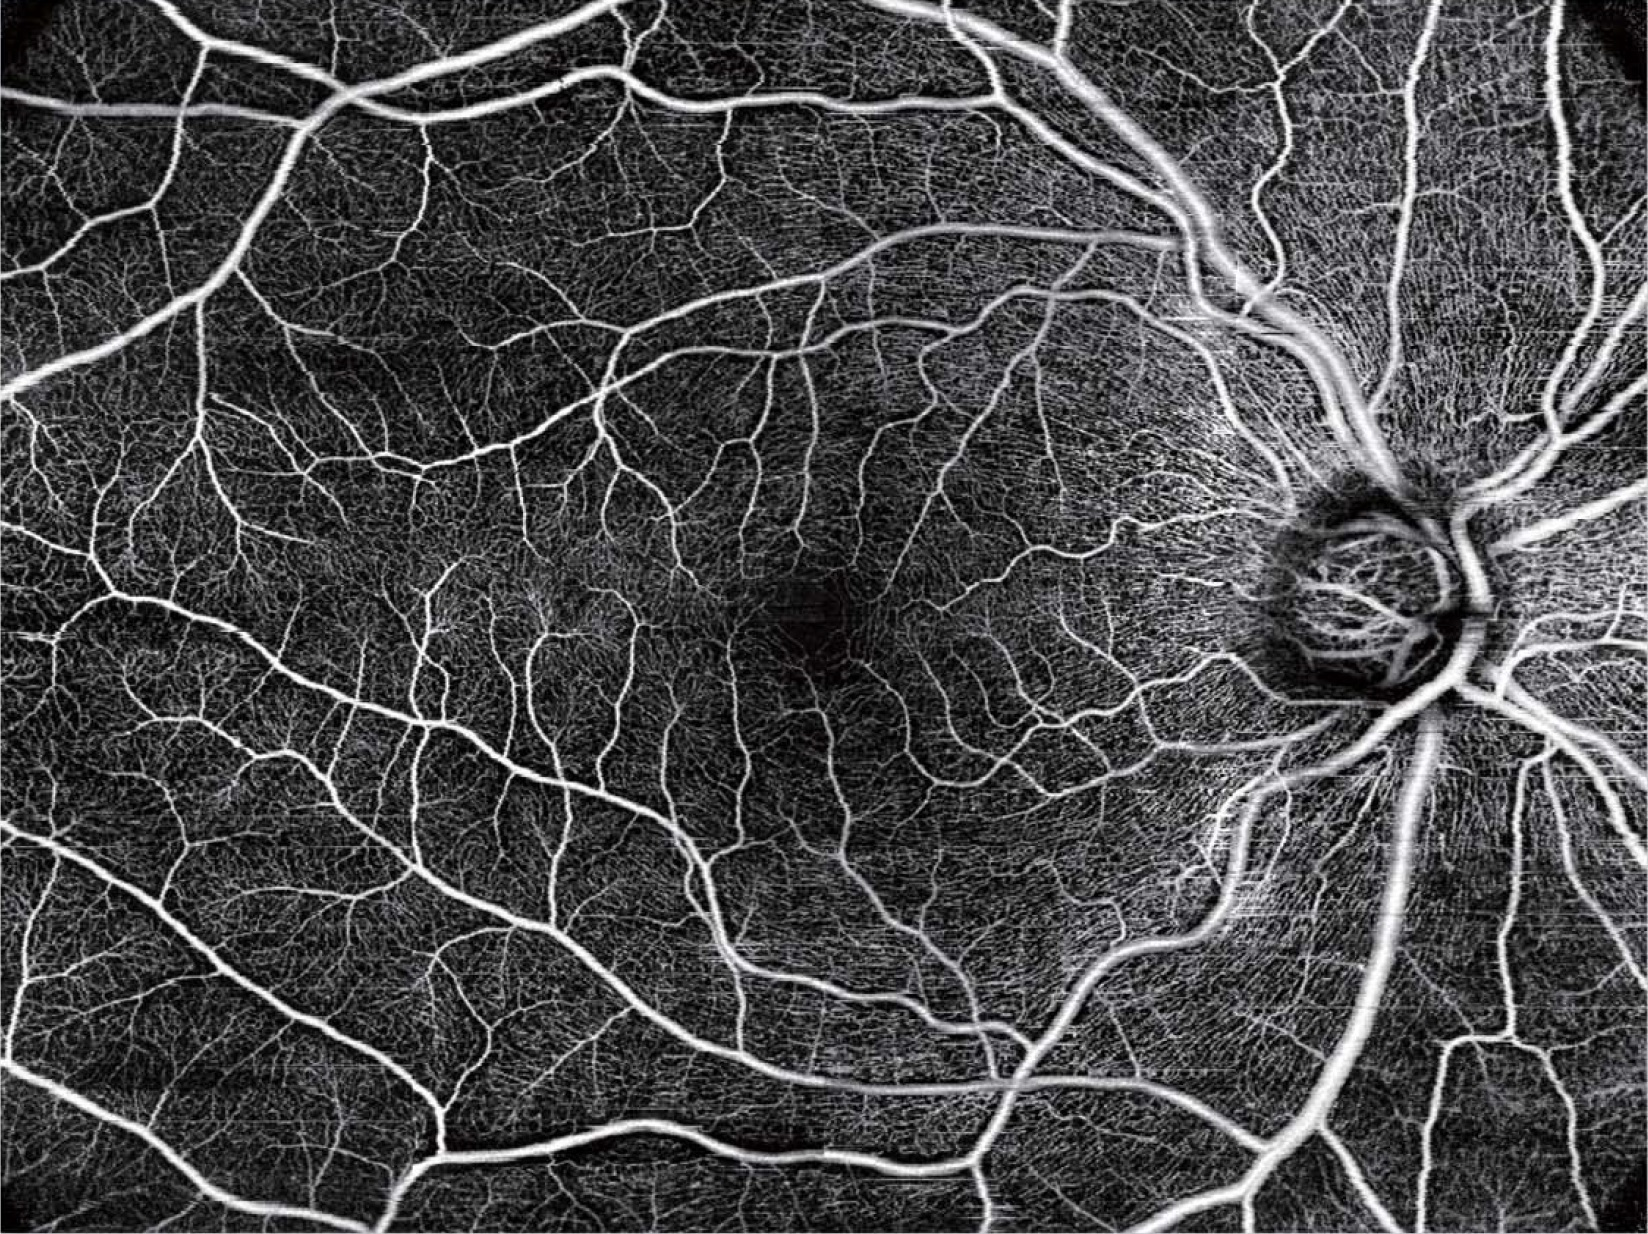
\includegraphics[width=0.3\textwidth]{figures/OCTA.jpg} % scale, width, height 
  \caption{Optical Coherence Tomography Angiography \cite{OCTA}}
  \label{fig:Glaucoma}
\end{figure}
\item \textbf{Fundus Photography}:is a method to screen the retina directly by using the pupil as the entrance and the exit of light rays for fundus camera.
The screening is achieved by placing the patient in front of the camera with the chin in a chin rest and the forehead against the bar.
Then, the photographer will align the camera and presses the shutter to fire a flash to create the fundus image\cite{sinthanayothin1999automated}.
Fundus images can be coloured with including some dyes like indocyanine and fluorescein.
\begin{figure}[htb]
        \centering
        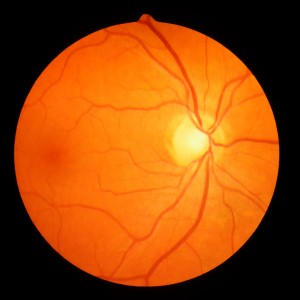
\includegraphics[width=0.3\textwidth]{figures/fundus.jpg} % scale, width, height 
  \caption{Fundus Photography \cite{fundus2016}}
  \label{fig:Glaucoma}
\end{figure}
\end{itemize} 

\section{Retina Analysis in OCT images}

In this section, previous work in the classification of the OCT images is presented and compared to have a better understanding of the field chosen.
Annotated data or dataset is required to diagnose the retina condition by analysing the retina morphology.
The design, implementation and testing of various previous work is reviewed.
There are many data for testing purposes and to be used with the permission of patients for scientific purposes.
Many datasets are available online for different parts or organs of the human body and also including the retina, where these datasets have different goals to study based on the case wanted to analyse.
The target in retina is different based on sickness needed to be diagnosed such as DME, AMD,DR, vessel segmentation and some localization tasks, hence many algorithms and datasets are done for each sickness to be diagnosed.
Since, the datasets are somehow useless if they are presented alone with no ground-truths aside the image or voxel to make the validation of the results and how accurate the designed algorithm.
By using the suitable method of image enhancing and extraction of data, ground-truth is giving a hand in training and testing data as the key to evaluate any algorithm's advantages and disadvantages.
This project used two types of data of OCT volumes, which they are SERI data and OPTIMA dataset.

\subsection{OCT Voxels Classification}
Over the past decades, the improvement in the applications of computer vision and image processing to
OCT volumes interpretation have been paid a big focus on improving an automated retinal layer
classification and segmentation methods.
This section discusses the recent state-of-the-art methods for classification using supervised and semi-supervised methods of SD-OCT volumes.
The datasets used in this study were acquired by the Singapore Eye Research Institute (SERI), using CIRRUS TM (Carl Zeiss Meditec, Inc., Dublin, CA) SD-OCT device \cite{cense2006ultra}.
The datasets consist of 32 OCT volumes (16 DME and 16 normal cases).
Each volume contains 128 B-scan with resolution of 512* 1024 pixels.
All SD-OCT volumes are read and assessed by trained graders and identified as normal or DME cases based on evaluation of retinal thickening, hard exudates, intraretinal cystoid space formation and subretinal fluid as presented in the table below.
Within the DME dataset, a large number of lesions were selected to create a rather complete DME dataset.
The volumes and sample numbers for DME volumes are presented in figure 2.4:
%\begin{figure}
%\centering
%        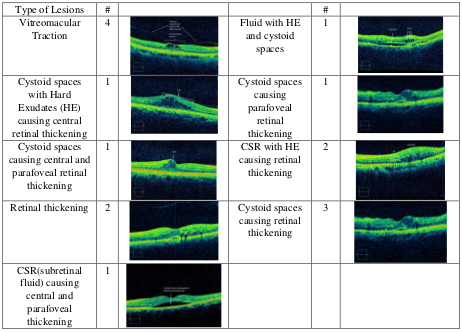
\includegraphics[width = 0.75\textwidth]{figures/bbdd.png} % scale, width, height 
%  \caption{Example of SERI dataset of DME}
%  \label{fig:SERI dataset}
%\end{figure} 

\begin{figure*}[t]
\begin{center}
   \subfigure[Vitreomacular traction.]{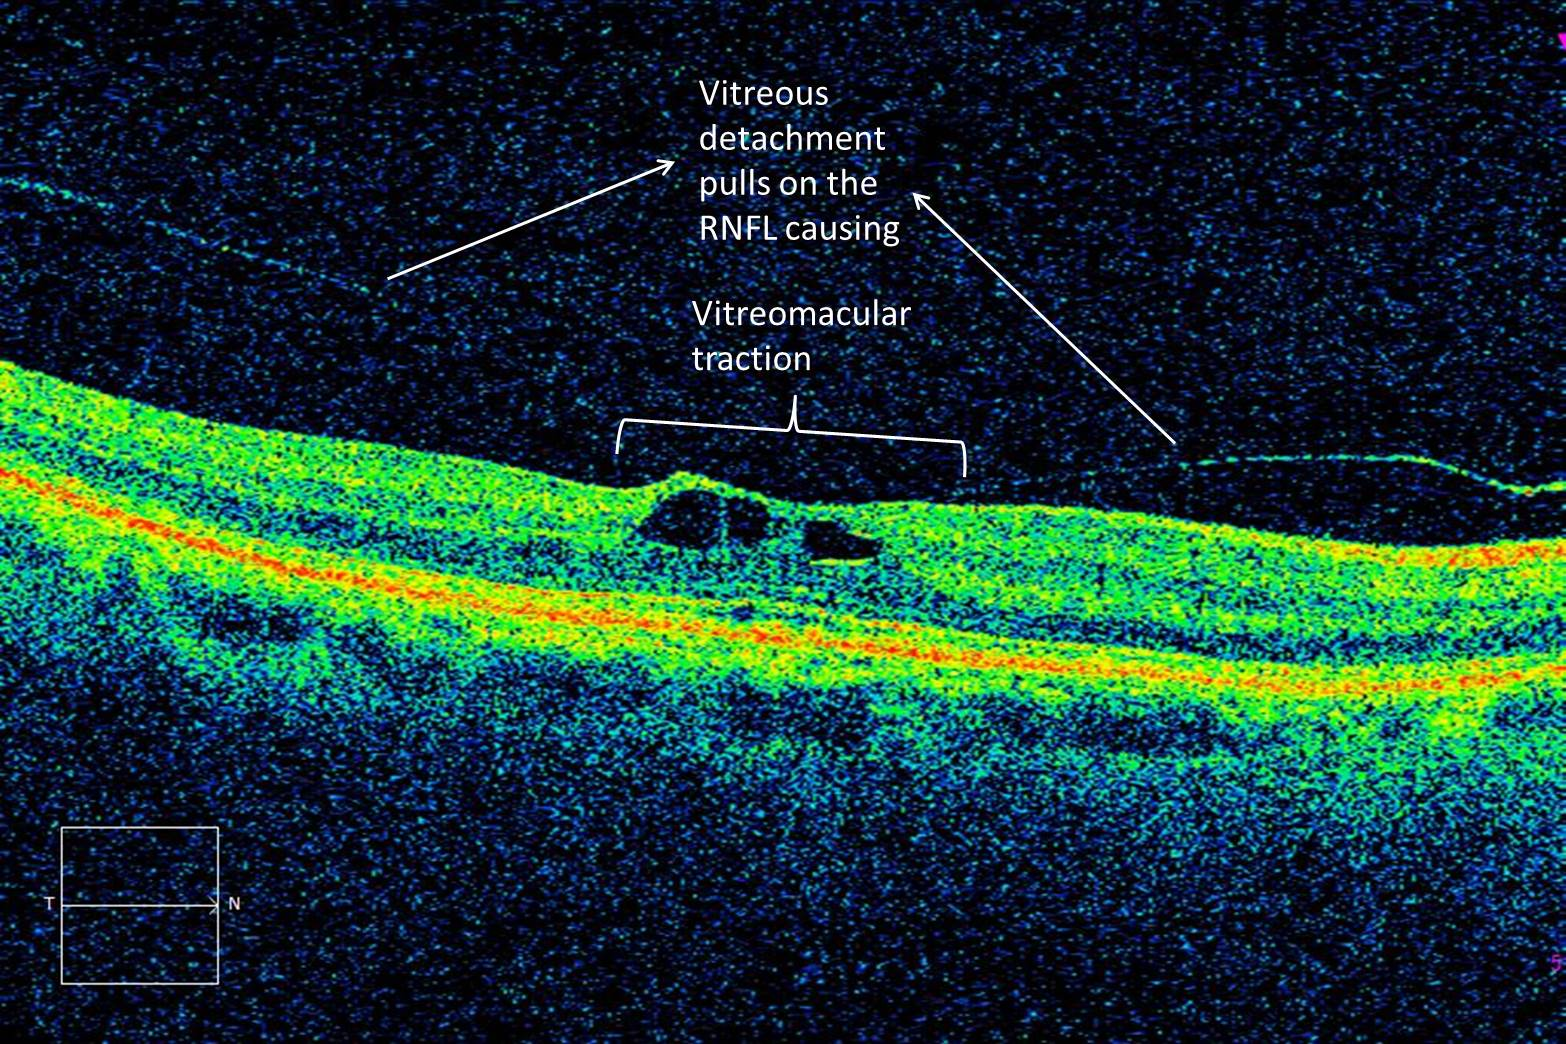
\includegraphics[width=0.3\textwidth, height = 0.15\textheight]{./figures/Vitreomacular}}\
   \subfigure[Rethinal thickening.]{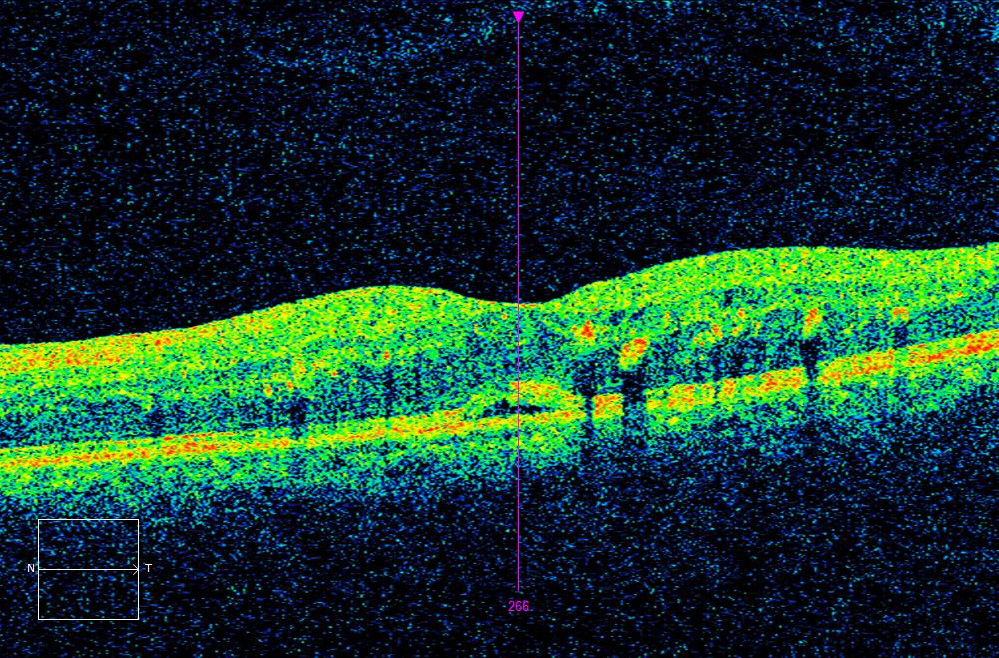
\includegraphics[width = 0.3\textwidth,height = 0.15\textheight]{./figures/RE}} \
   \subfigure[Cyst spaces, causing central and parafoveal retina thickening.]{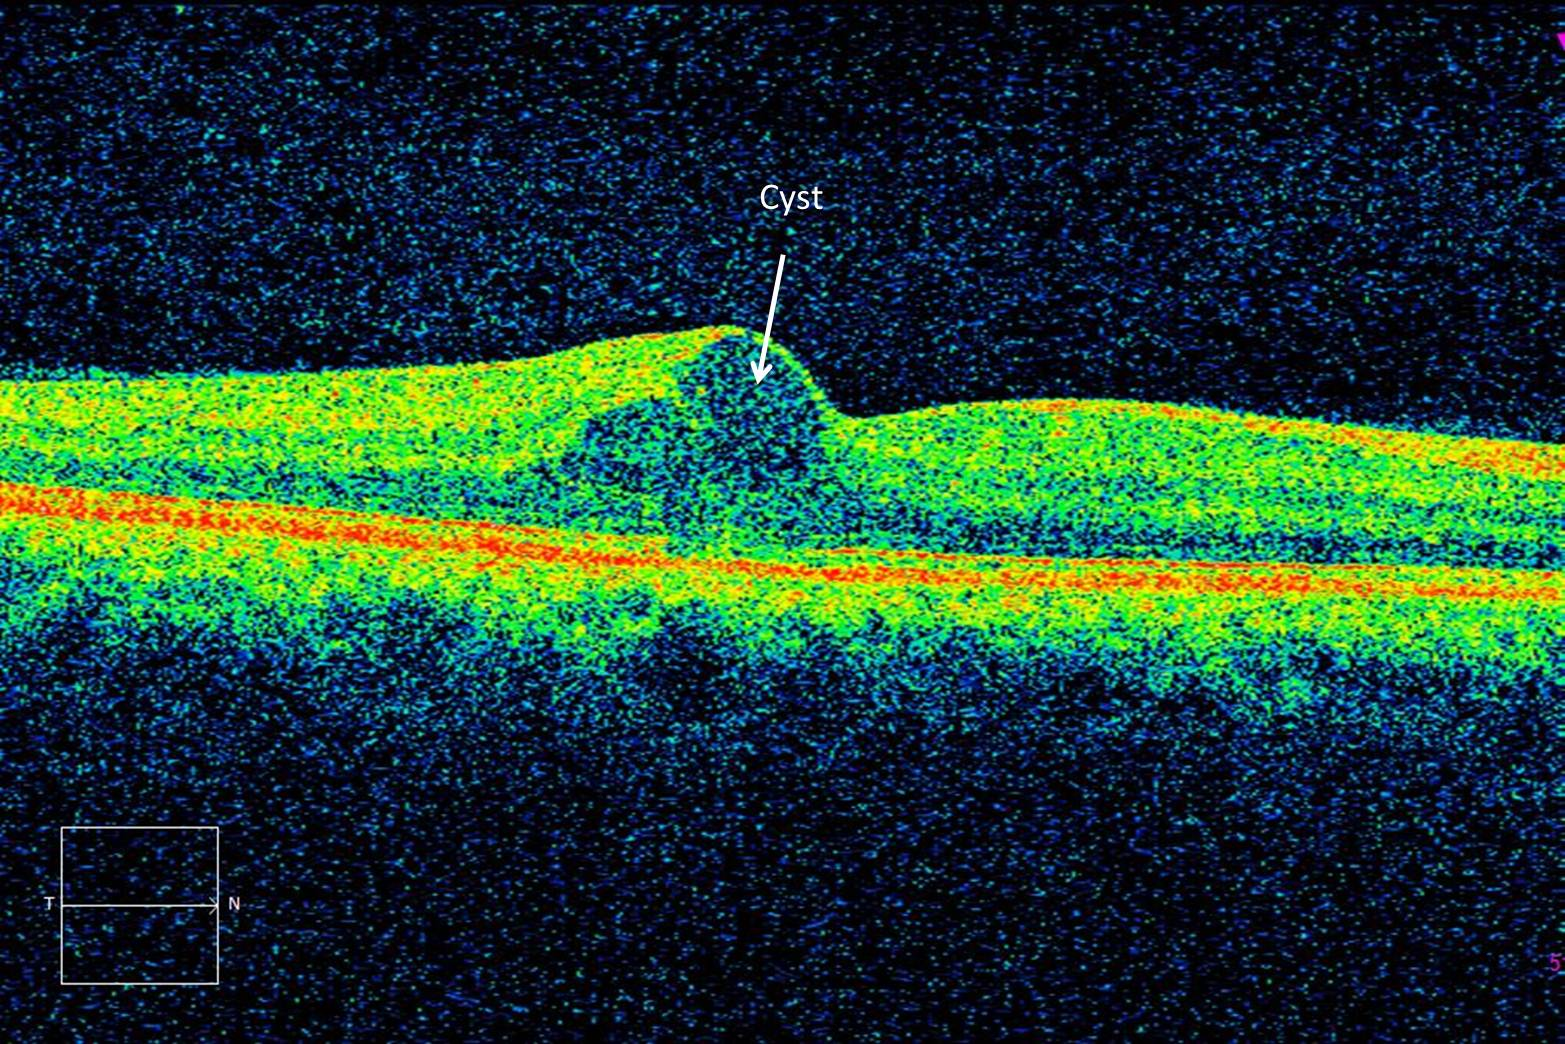
\includegraphics[width=0.3\textwidth,height = 0.15\textheight]{./figures/Cyst}}\\
   \subfigure[Cyst spaces and hard exudates, causing central retinal thickening.]{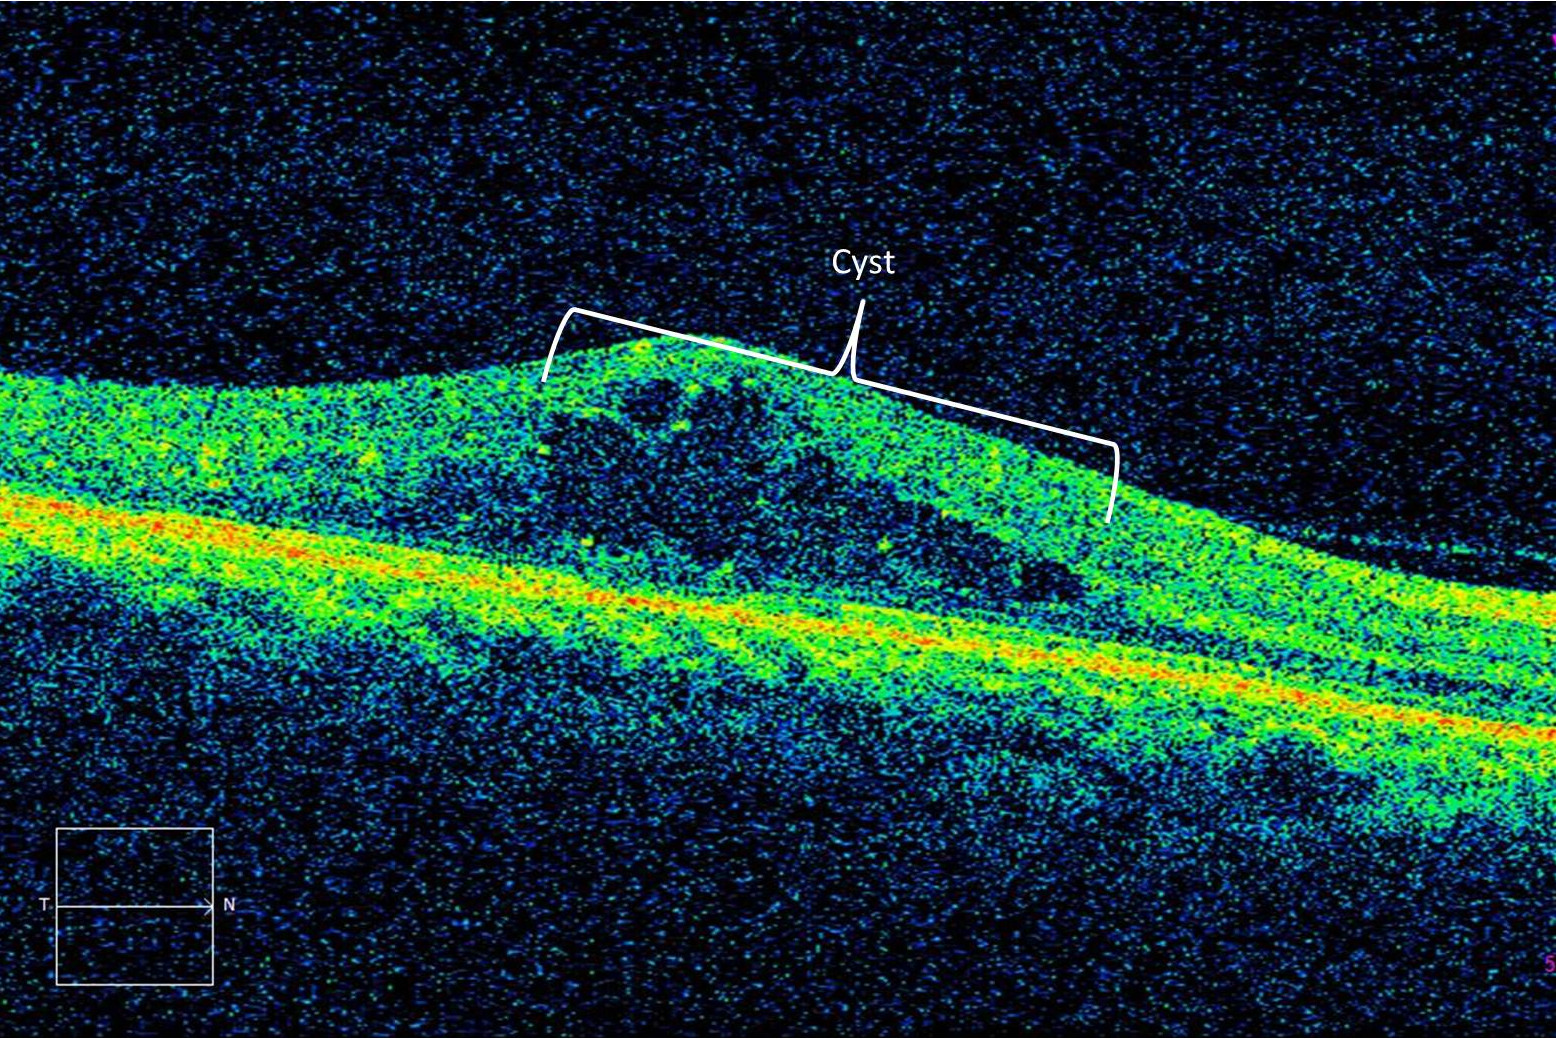
\includegraphics[width = 0.3\textwidth,height = 0.15\textheight]{./figures/Cyst+HE+RE}} \
   \subfigure[CSR (subretinal fluid), causing central and parafoveal thickening.]{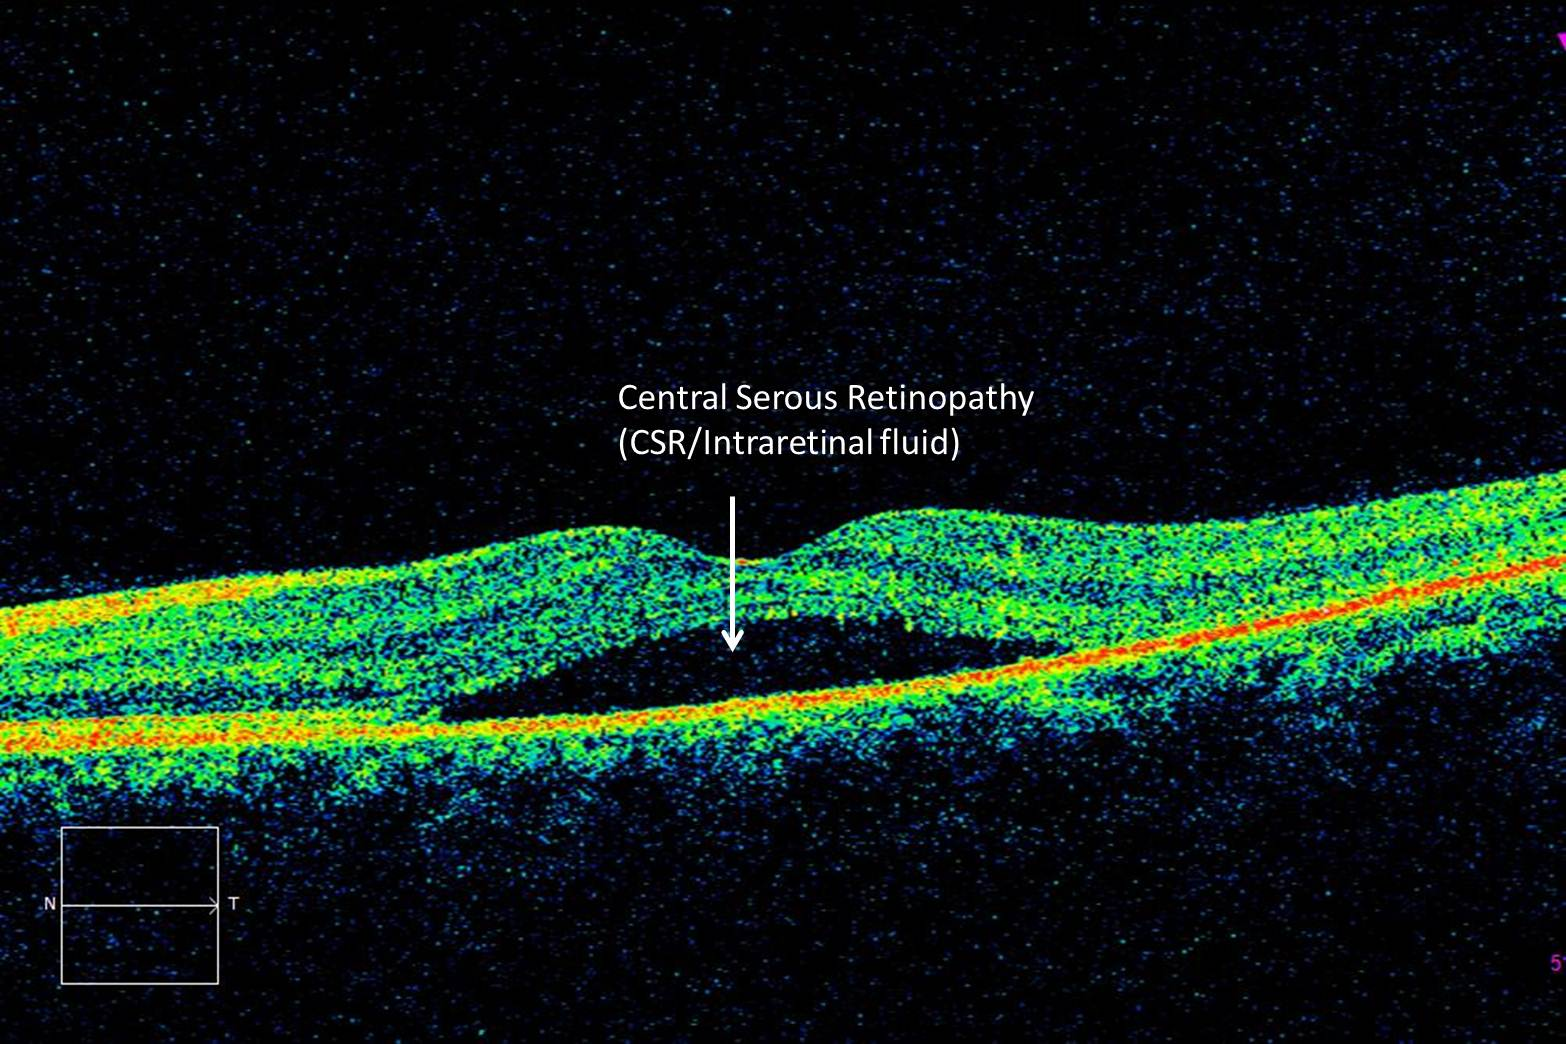
\includegraphics[width = 0.3\textwidth,height = 0.15\textheight]{./figures/CSR}} \
   \subfigure[CSR, hard exudates and cyst spaces.]{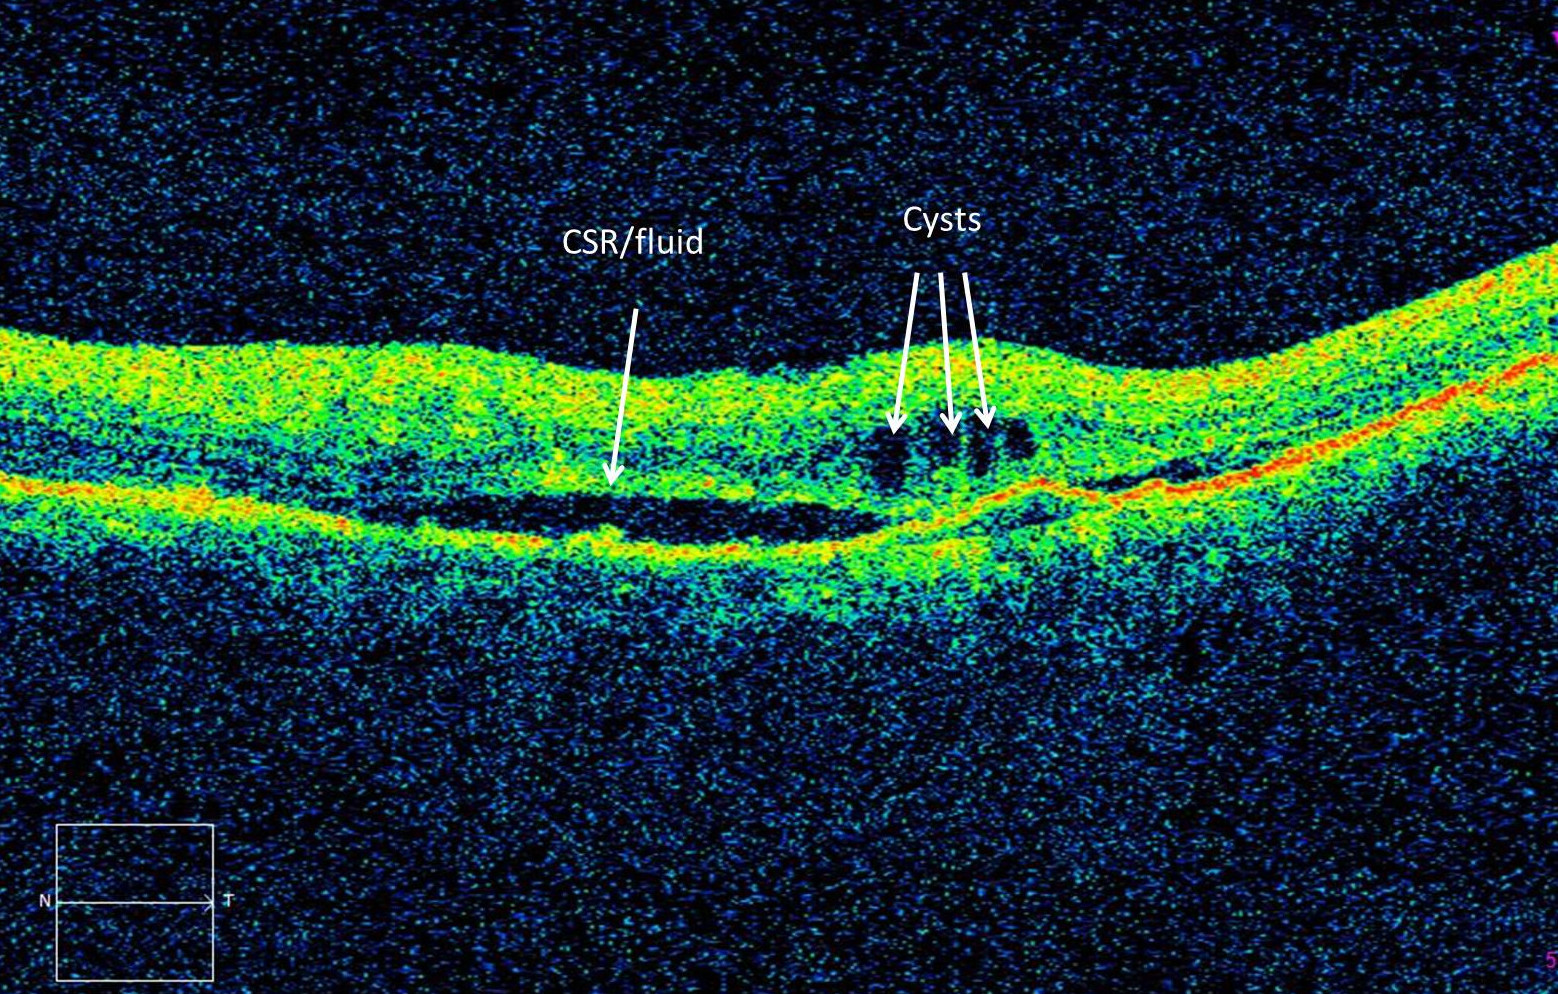
\includegraphics[width = 0.3\textwidth,height = 0.15\textheight]{./figures/Cyst+CSR+HE}} \\
   \subfigure[Cyst spaces, causing retinal thickening.]{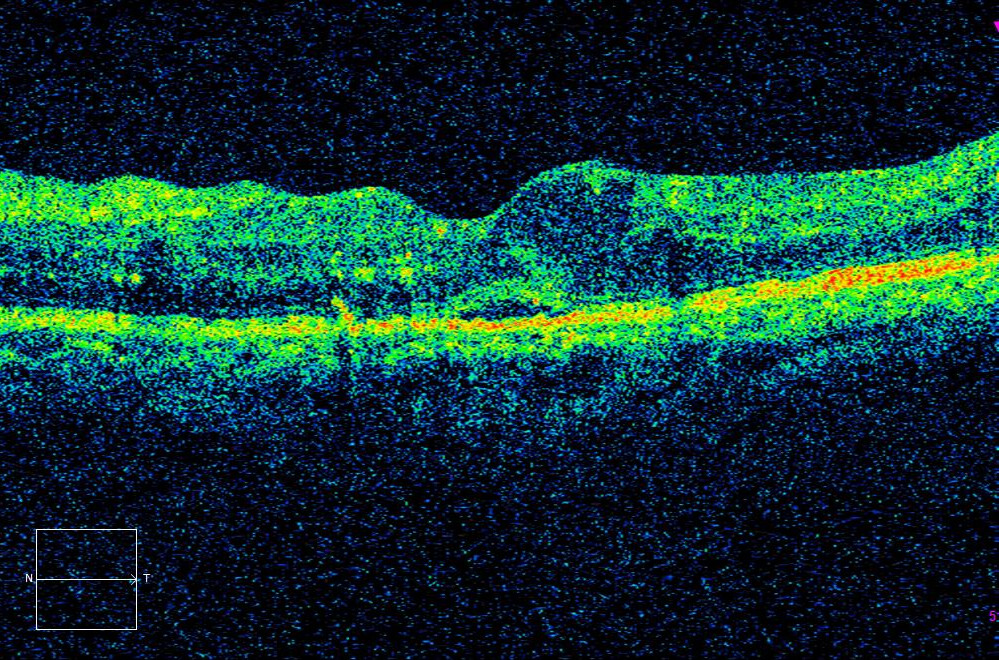
\includegraphics[width = 0.3\textwidth,height = 0.15\textheight]{./figures/Cyst+RE}} \
   \subfigure[CSR and hard exudates, causing retinal thickening.]{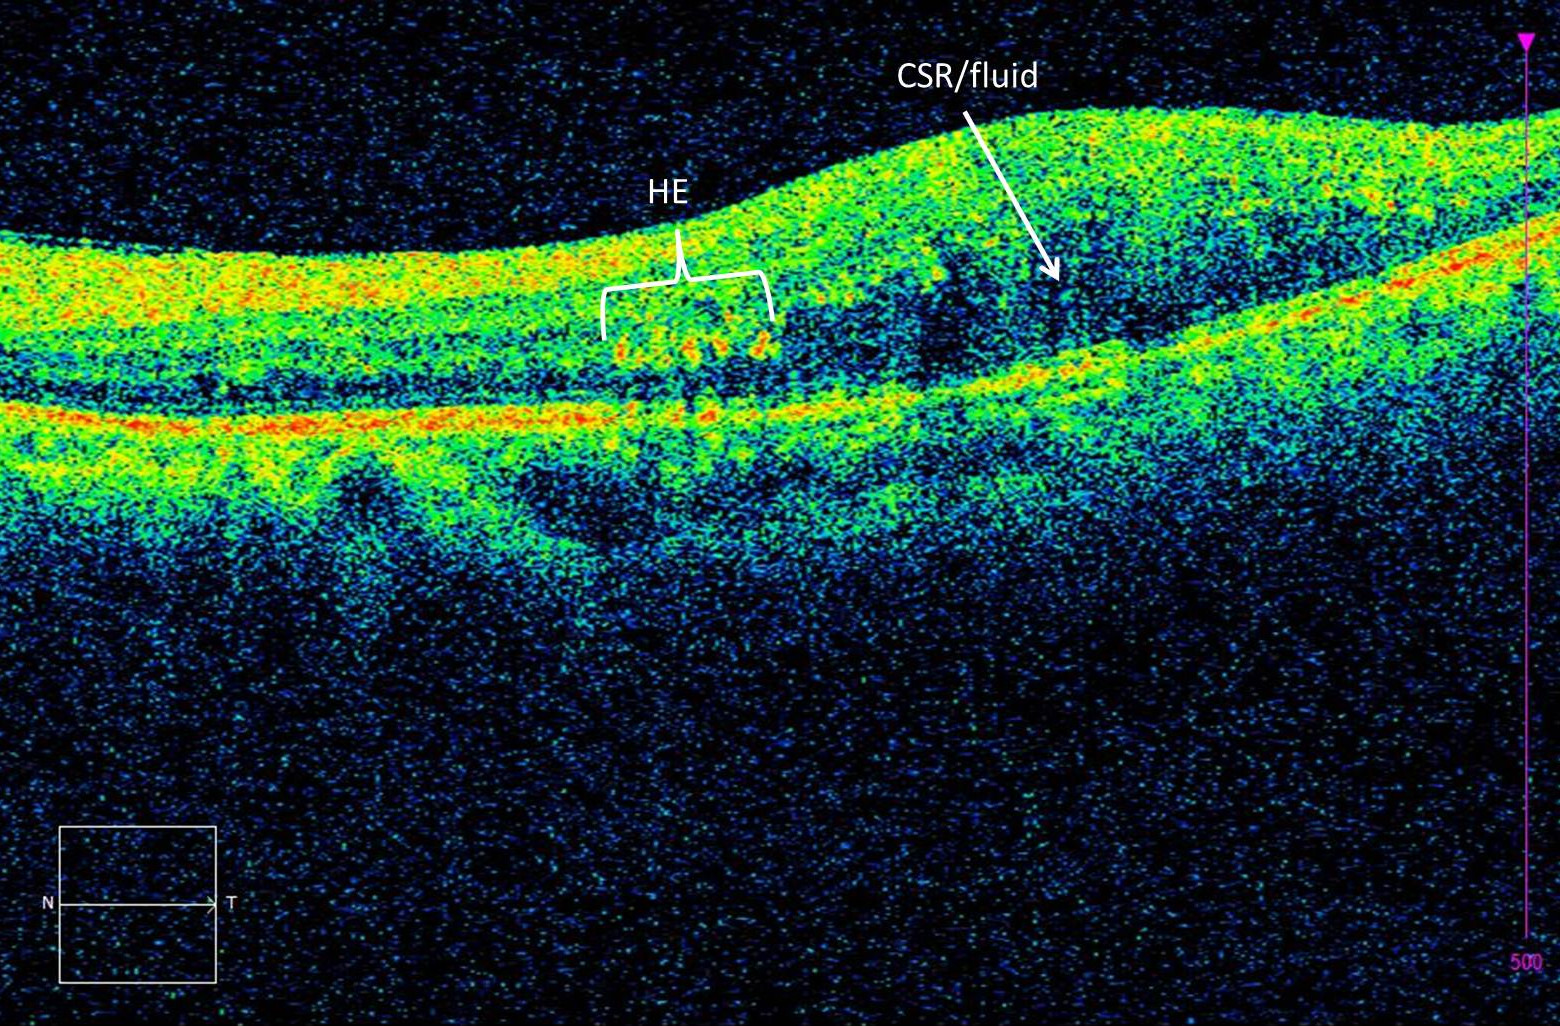
\includegraphics[width = 0.3\textwidth,height = 0.15\textheight]{./figures/CSR+HE+RE}} \   
   \subfigure[Cyst spaces causing parafoveal thickening.]{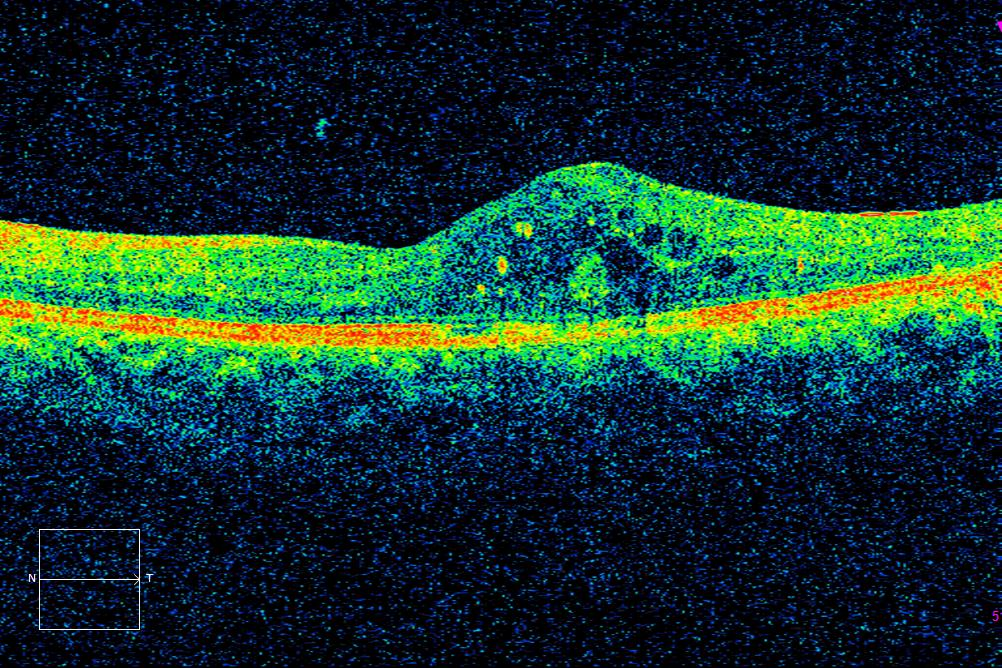
\includegraphics[width = 0.3\textwidth,height = 0.15\textheight]{./figures/Cyst+RE_parafovel}} \\
    
\end{center}
    \caption{Examples of \acs{dme} cases in \acs{seri} dataset.}
  \label{fig:bbdd}
\end{figure*}

Before, heading straight away to the algorithm, we shall know what is Machine learning.
Inventors have long dreamed and though of creating machines that are able to think just like humans.
The difficulties might face any systems depending on hard-coded knowledge said that Artificial Intelligence systems acquire the ability to have their own knowledge, by extracting features in patterns from raw data.
This capability is known as machine learning, essentially a form of applied statistics.
To have a precise definition we define what learning is first.
Learning is provided by \cite{mitchell1998introduction} \' A computer program is said to learn from experience E with respect to some class of tasks T and performance measure P, if its performance at tasks in T, as measured by P, improves with experience E\' .
And a human can imagine how computer can integrate couple of experiences, tasks and performances based on how powerful the computer is used for the particular task.
Tasks in machine learning can be classification, classification with missing inputs, regression, transcription, anomaly detection and many others. 

Srinivasan et al. propose a classification method to distinguish normal, DME, and Age-related Macular Degeneration (AMD) OCT volumes \cite{srinivasan2014fully}.
The SD-OCT volumes are enhanced by: 
\begin{itemize}
\item reducing the speckle noise through a de-noising method, which enforces the sparsity in a specific transform-domain.
\item flattening the retinal curvature.
\end{itemize}  
After that, edge information is extracted using Histogram of Oriented Gradients (HoG)descriptor for each B-scan of a volume and later used to train a linear Support Vector Machine (SVM).
This method is evaluated on a dataset of 45 patients equally subdivided into the three mentioned classes and led to a correct classification rate of 100\%, 100\% and 86.7\% for normal, DME and AMD
patients, respectively.
The dataset used by \cite{srinivasan2014fully} is publicly available but is already pre-processed (i.e., denoised, flattened, and cropped).
Furthermore, this dataset does not offer a huge variability in terms of DME lesions, have different sizes for the OCT volumes, and some of them, without specifying which, have been excluded during the training.
All these reasons, prevent us from using this dataset to benchmark our work.

Venhuizen et al. recently proposed a method to classify AMD and normal OCT volumes in \cite{venhuizen2015automated} using Bag of Words (BoW) models.
In the proposed method, the features are extracted from a set of key-points detected from each individual B-scan.
As a feature descriptor, a 9 px × 9 px texton is extracted around each selected key-point and its dimension is reduced, from 81 to 9 using Principal Component Analysis (PCA).
A dictionary or codebook is created by clustering the features extracted and each volume is represented in terms of a histogram, which captures the codebook occurrences.
These histograms are used as a final feature vectors to train a Random Forest (RF classifier.
This classifier is evaluated on a dataset composed of 384 volumes leading to an Area Under the Curve (AUC) of 0.984.

Liu et al. propose a methodology for detecting macular pathology in OCT images using Local Binary Pattern (LBP) and gradient information as attributes \cite{liu2011automated}.
Each B-scans is aligned and flattened and a 3-level multi-scale spatial pyramid is created. Additionally, edges are detected using Canny detector on the same pyramid.
Subsequently, an LBP histogram is extracted for each of the layer of the pyramid.
All the obtained histograms are concatenated into a global descriptor whose dimensions are reduced using PCA.
Finally, a SVM with an Radial Basis Function (RBF) kernel is used as classifier.
The method achieved good results in detection of OCT scan containing different pathology such as DME or AMD, with an AUC of 0.93 using a dataset of 326 OCT scans.

Lema\^{i}tre et al. propose another method based on extracted LBP features from OCT images and dictionary learning using BoW models \cite{lemaitre2015classification}. Contrary to \cite{srinivasan2014fully}, BoW and dictionary learning are used to perform volume classification is performed rather than B-scan. In this method, the OCT images are first pre-processed using Non-Local Means (NLM) filtering to reduce the speckle noise.
Then, the volumes are mapped into discrete set of structures namely: local, when these structures correspond to patches; or global, when they correspond to volume slices or the whole volume.
According to different mapping, LBP or Three Orthogonal Planes (LBP-TOP) texture features are extracted and represented per volume using histogram, PCA, or BoW.
The final feature descriptors per volumes are classified using RF classifier.
Classifying DME versus normal volumes on a balanced dataset of 32 SD-OCT volumes, the classification performance in terms of sensitivity (SE) and specificity (SP) of 87.50\% and 75\%, respectively, is achieved, while using LBP-TOP features and global mapping.

On the same dataset, Sankar et al. proposed a rather different approach, based on semi-supervised learning, to address the issue of an anomaly detection \cite{sankar2016classification}.
In their method, the authors proposed a technique that does not only allow the classification
of the OCT volume, but also enables the identification of the abnormal B-scans inside the volume.
This approach is based on modelling the appearance of normal OCT images with a Gaussian Mixture Models (GMM) and detecting abnormal OCT images as outliers.
The classification of an OCT volume is based on the number of detected outliers.
Testing on 32 OCT volumes, their proposed method achieved SE and SP of 93\% and 80\%, respectively.
A conclusion of this techniques is presented on table 2.1

\begin{table*}[t]
\caption{Summary of the state-of-the-art methods.}
\resizebox{1\linewidth}{!}{
\begin{tabular}{l ccc c cccc	c c c c	c c}
\toprule
References & \multicolumn{3}{c}{Diseases} & Data  & \multicolumn{4}{c}{Pre-processing} & Features & Representation & Classifier & Evaluation & Results\\
    &  &  &  & size &  &  &  &  &  &  &  & & &\\
   \cmidrule(l){2-4}\cmidrule(l){6-9} 
    & \acs*{amd} & \acs*{dme} & Normal  &           & De-noise & Flatten & Aligning & Cropping &   & &   &  &   \\
\midrule
& & & & & & & & & & & & & &  \\
Srinivansan~\textit{et~al.}~\cite{srinivasan2014fully} & $\checkmark$ & $\checkmark$ & $\checkmark$ &  45 & $\checkmark$ & $\checkmark$ &  & $\checkmark$ & \acs*{hog} &  & linear-\acs*{svm} & \acs{acc} & 86.7\%,100\%,100\%  \\
& & & & & & & & & & & & &    \\
Venhuizen~\textit{et~al.}~\cite{venhuizen2015automated} & $\checkmark$ &  & $\checkmark$ & 384 &  & & & &  Texton  &\acs*{bow}, \acs*{pca}  & \acs*{rf} & \acs*{auc} & 0.984 \\ 
& & & & & & & & & & & & &   & \\
Liu~\textit{et~al.}~\cite{liu2011automated} & $\checkmark$ & $\checkmark$ & $\checkmark$  & 326 &  & $\checkmark$ & $\checkmark$ &  &  Edge, & \acs*{pca}& \acs*{svm}-\acs*{rbf} &\acs*{auc} & 0.93 \\
& & & & & & & & &\acs*{lbp} & & & & \\
& & & & & & & & & & & & &  \\
Lema\^itre~\textit{et~al.}~\cite{lemaitre2015classification} &  & $\checkmark$ & $\checkmark$ & 32  & $\checkmark$ &  &  &  & \acs*{lbp}, & \acs*{pca}, \acs*{bow}&  \acs*{rf} & \acs*{se},\acs*{sp} & 87.5\%, 75\%  \\
& & & & & & & & &\acs*{lbptop} & Histogram & & &  \\
& & & & & & & & & & & & &  \\
Sankar~\textit{et~al.}~\cite{sankar2016classification} & & $\checkmark$ & $\checkmark$ & 32 & $\checkmark$ & $\checkmark$ & & $\checkmark$ & Pixel & \acs*{pca} & Mahalanobis & \acs*{se}, \acs*{sp} & 80\%, 93\% \\
& & & & & & & & &-intensities & &-distance to \acs*{gmm} & & \\ 
& & & & & & & & & & & & &  \\
\bottomrule
\end{tabular}}
\label{tab:survey-tab}
\end{table*}

\subsection{OCT Patch or Cyst Classification}
This section aims to explain the state of arts of work done in segmenting OCT voxels.
Inspired from the research done in segmenting OCT images, we did the classification on potential regions.
The SD-OCT data used in this project is provided by the OPTIMA laboratory (Christian Doppler Laboratory for Ophthalmic Image Analysis, Department of Ophthalmology, Medical University of Vienna) for the Cyst segmentation challenge hosted at MICCAI 2015.
These data consisted of 15 SD-OCT volumes containing a wide variety of retinal cysts with accompanying clinical ground truth annotation manually drawn by two different experts (Two Ground-Truths).
The SD-OCT voxels have 4 different vendors at different resolutions and scanning patterns: four volumes from Cirrus (Carl Zeiss Meditec, Dublin, CA, USA), three volumes from Nidek (NIDEK Co., Hiroishi, Gamagori, Japan), four volumes from Spectralis (Heidelberg Engineering, Heidelberg, Germany) and four volumes from Topcon (Topcon medical Systems,Santa Clara, CA, USA).
Results validation in this challenge were compared with the first and second reading by experts and the intersection between them compared to the segmented method done by the researcher.
Some examples of the Data used by Optima as shown in figure 2.16:
\begin{figure*}[t]
\begin{center}
   \subfigure[Cirrus-1.]{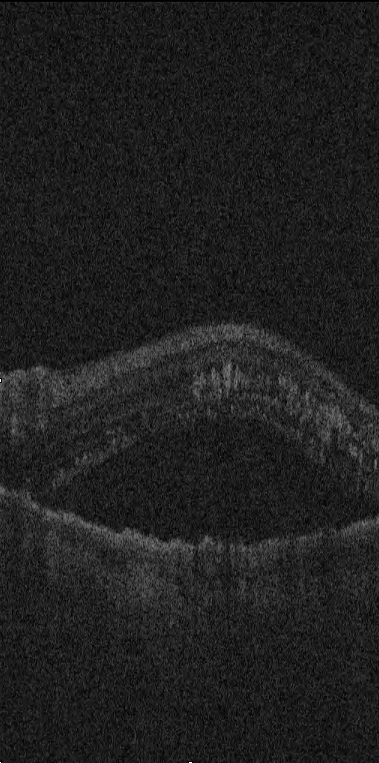
\includegraphics[width=0.4\textwidth, height = 0.2\textheight]{./figures/Cirrus_1.png}}\
   \subfigure[Nidek-1.]{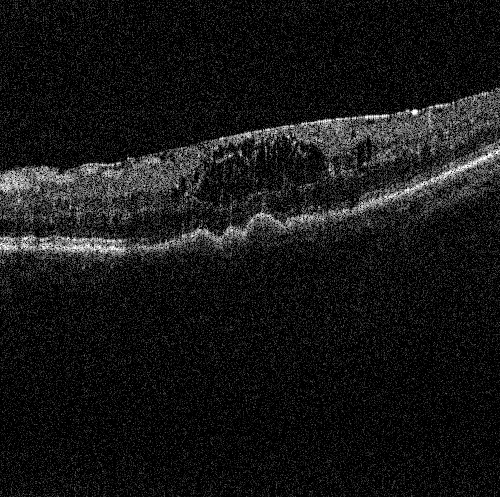
\includegraphics[width = 0.4\textwidth,height = 0.2\textheight]{./figures/Nidek_1.png}} \\
   \subfigure[Spectralis-1.]{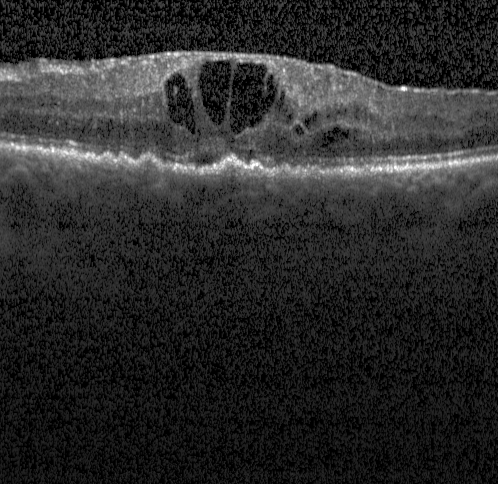
\includegraphics[width=0.4\textwidth,height = 0.2\textheight]{./figures/Spectralis_1.png}}\
   \subfigure[Topcon-1.]{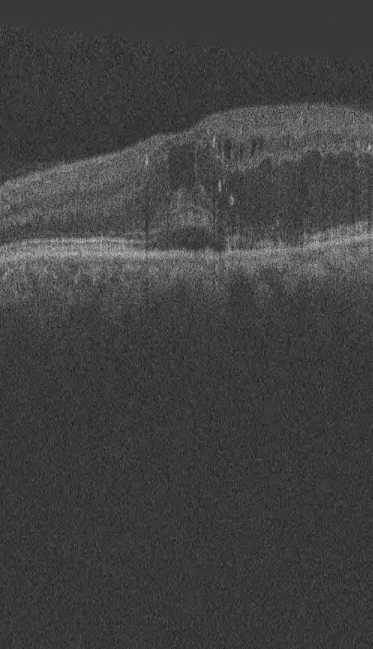
\includegraphics[width = 0.4\textwidth,height = 0.2\textheight]{./figures/Topcon_1.png}} 
   
\end{center}
    \caption{Examples of \acs{dme} and \acs{amd} cases in OPTIMA dataset.}
\end{figure*}

Many researchers went through this challenge made by Optima laboratory.
The method proposed by Luis et al \cite{LuisdeSisternes2015Optima} is a machine learning based, where a model is trained using manual markings (to establish the ground truth) and then tested using another 15 volumes of testing data also provided by OPTIMA laboratory.
In the preprocessing stage, the SD-OCT data normalized and de-noised using non-local means filtering in the axial and horizontal direction.
A defined number of boundaries defining the axial location of defined intra-retinal layers are then automatically outlined using a developed segmentation algorithm done by Luis et al in \cite{de2015localization} (SOARS: Stanford OCT Automated Retinal Segementation).
A number of quantitative features (34 features) are extracted to characterize each volume located between the segmented internal limiting membrane (ILM) and inner segment junction (IS), where the possible cysts are located in.
These features expanded to have four possible resolutions using multi-resolution approach to have set of predictors. 
After that, they calculate the risk score for each voxel.
The final segmentation output is generated automatically by detecting an adaptive threshold to
stratify the output scores in those belonging to a cyst or background.
The accuracy using this method has achieved a good results using dice coefficient evaluation with 80\% of correctly segmenting the B-scan slices.

Another proposed method by Ipek et al., \cite{oguz2016optimal}, which is using cost
function (opposed to machine-learned) that generalizes well to a variety of images.
This cost function takes into account the general characteristics of the input image as well as the well-known characteristics of fluid-associated abnormalities.
As the background and the cyst color in OCT images is black, so all methods care about certain area of the B-scan slice which lies between the layers.
They create a reliable mask even with the presence of fluid associated with cysts, followed by using a method to correct the Bruch membrane (BM). 
Then they segment using a cost function and they compare with the experts results.
This method fully cover all black holes lie in the layers and they did not target cysts only.

Mahdad et al., \cite{Mahdad2015Optima} used a speckle noise reduction algorithm, which maintains strong edge sharpness and reduce the noise.
This can be achieved by applying recursive Gaussian filter to noisy images and to any zero pixel exist in the image.
After that, threshold is used to the image to segment fluid space pixels.
Then nerve fibre layer (NFL) and retinal pigment epithelium (RPE) layer are extracted in each B-
scan.
Finally, most of the possible false positives (FPs) are removed based on standard deviation and morphology of extracted candidate pixels.

Another proposed method by Karthik in \cite{Karthik2015Optima} to segment OCT images.
They started by de-noising the image by using Total Variational approach that will reduce the texture content resulting in a smooth piecewise constant images preserving the edges.
Then, the make candidate selection as all methods done to specify the process only between NFL and RPE to save time and avoid pixels that they have nothing to do with the assessment of the disease existed in the voxel.
After that, Candidate regions are extracted using Maximally stable extremal regions(MSER).
This feature computation produces a set of stable region in an image.
MSER also used to detect the multi-scale objects without any smoothing.
Both small and large structure can be detected based on threshold and other aspects based on the favoured regions wanted to be extracted.
Then, based on the texture of pattern calculation, a local descriptor is assigned to each batch after making a bounding box for each region extracted by MSER.
Finally , with fifty trees in Random forest classifier is used for results validation and the results were challenging as it gives good results when the cyst is in medium and large size and poor results for small cysts.

A novel method using different way of training and extracting data proposed by Venhuizen \cite{venhuizen2015autCNN}.
His method mainly using the Convolution Neural Network to segment the images.
Two stages define the process, in the first stage, Three convolution neural networks (CNNs) are used to get a segmentation at different image scales.
In the second stage, the three CNNs scale segmentations are fused together, redefining the borders of the segmented cysts by combining local information obtained with the lower scale network with contextual information obtained from the higher scale networks.


%An image correspondence method is based on finding a mapping
%function ($f(x,y)$) that maps each coordinate of one image ($A$)
%into another image ($B$).

%\begin{equation}
%B(x',y')=A(f(x,y))
%\end{equation}
%\noindent  $B$.  $f_x$ and $f_y$(and $f_z$). 


%$m=(x',y')$ to its nearest point:
%
%\begin{equation}
%        B(m)=\sum_iw_i B(n_i)
%\end{equation}
%\noindent where each weight $w_i$ is related to the distance from
%$m$ (see Figure~\ref{fig:interp})
%
%\begin{equation}
%        w_1 = (1-dx)(1-dy) ~~~~ w_2 = (1-dx)dy ~~~~w_3 = dx(1-dy)
%        ~~~~ w_4 = dx dy
%        \nonumber
%\end{equation}


\chapter{Methodology} \label{chap:Methodology}

There are many unpredicted aspects that can result in unwanted images in real world screen environment.
For this reason, many algorithms were reviewed in the previous section to give an idea of the project scope.
Preprocessing step is a must to have better results and to get clear image to specify the disease and have an algorithm to track it.
For some drawbacks in the algorithms reviewed regarding accuracy, speed and sensitivity and etc, we have introduced an automatic algorithm to classify the OCT volumes based on the Data provided SERI and OPTIMA.
Another algorithm is introduced in the project, which segmenting the OCT images using the auto-encoder.
In this chapter, we present the method for both algorithms.
A MATLAB code implementation is developed using the cluster provided by University of Burgundy with Xeon 2630 V3 processor, 128 GB of RAM and a GPU Nvidia Tesla K40 which processes the algorithm proposed starting from 10 minutes to 9 hours of some detailed tasks.

\section{Introduction}

Many systems for retinopathy automatic detection in OCT images have been improved.
The results obtained is promising and discussed in the next chapter.
The machine used to train this system proposed is powerful to process a very big data in some hours where normal computers might take days to weeks to achieve the same task.
Algorithm used to correct the images light or contract increasing is used in the pre-processing section.
However, the image enhanced has limited resolution obtained cause sometimes increasing the threshold will yield to over-blurring , which is not good due to info losing might be useful.
Feature extraction in the images is also taking time to process meanwhile the multi-pyramid way is used.
In addition to those, feature representation is used to have a clear dictionary to the classifier.

Accuracy quality is a subjective concept to be determined.
It is not a straight task to be determined and this can be noticed with the different experts opinions  in term of making a decision of the same aspect.
To detect a disease that attacks the eye, same imaging technique is useless.
The reason behind that, in Glaucoma we need dark images to better figure out the nerves problem, while dark images are considered low quality if we want to detect Diabetic Retinopathy(DR).
Hence, we used confusion Matrix based on how many volumes detected as Normal, DME or wrong for both cases for the first part of the Project.

The second part, is using deep learning technique to train the data after extracting the data using the MSER features to cover the cyst.
The segmentation done by assigning a label to the cyst location then fitting it to the auto-encoder then we have a test data with their ground truths to be sent for prediction based on the cluster created from the auto-encoder.
Accuracy decision is made based on Dice coefficient and compared with the two ground truth provided by OPTIMA laboratory and the intersection between them.  

Processing speed is another aspect to be taken into account when processing the algorithms, hence a powerful computer is in need for decision making about detecting diseases.
This chapter explains the methodology of the algorithms and it is divided into two parts, first is OCT classification and the second is the OCT segmentation. 

\section{Automatic classification Of OCT Volumes}

Inspired by the previous methods and using machine learning tools to obtain an automatic machine able to make a decision.
A supervised learning algorithm is designed to map a certain function with a known inputs and outputs.  
Our classification pipeline is depicted in Fig.3.1.
The rest of the section present into details each intermediate step.
Our approach is based on the original paper of Srinivasan et al\cite{srinivasan2014fully}.
It has been enhanced with feature representation like PCA , proposed in  \cite{venhuizen2015automated} and BoW.
Different classifiers are used and the results presented in the next chapter

\begin{figure}[htb]
        \centering
        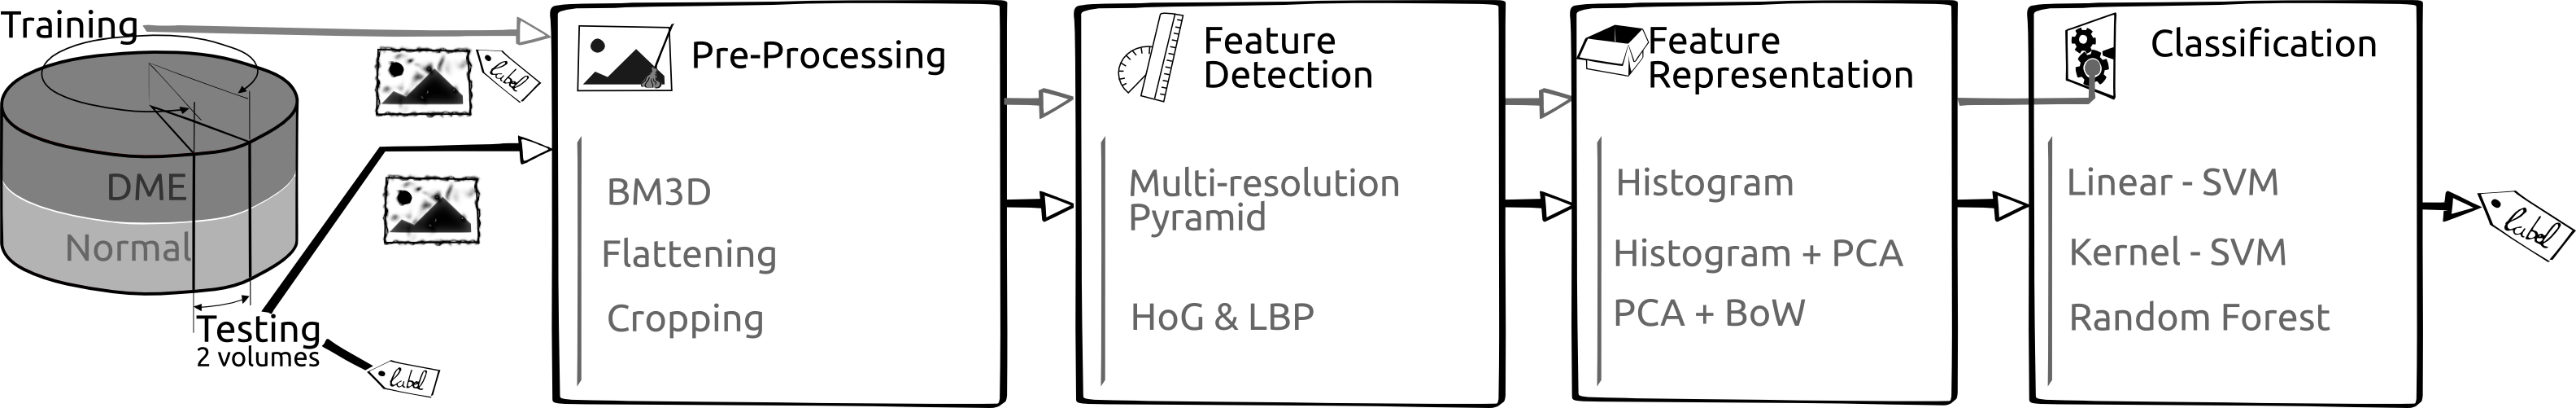
\includegraphics[width = 1.2\textwidth]{figures/Khaled-ICPR-method.png} % scale, width, height 
  \caption{Classification Pipeline}
  \label{fig:Classification Pipeline}
\end{figure} 

\subsection{Preprocessing}

Image blurring and sharpening is essential and critical step in machine learning aspects to ensure the high quality of the data presented to by analysed in a process called preprocessing.
Fixing the imperfections in the images is important to let the following tools useful.
So, this process is the main basis of images processing field. 
This project introduces the first step as Preprocessing as shown in the figure 3.2.
A sample of the image is shown here:
\begin{figure}[htb]
        \centering
        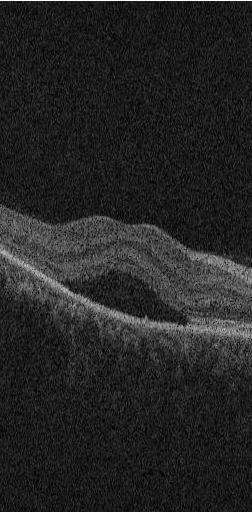
\includegraphics[width = 0.3\textwidth, height = 0.2\textheight]{figures/Original-image.jpg} % scale, width, height 
  \caption{Original B-scan slice}
  \label{fig:Original image}
\end{figure}

Following the work done by Srinivasan et al. \cite{srinivasan2014fully},and prior to feature extraction, the OCT volumes are pre- processed through de-noising, flattening, and cropping steps, the details as follow:
\begin{enumerate}
\item \textbf{De-noising}:It is the process of affecting the look of a certain image, by modifying pixels and its neighbours by some math equations applied to the images matrices.
Applying some filters to a particular images to enhance the look and remove the noise away.
In this part of the project we have used Block Matching 3D filtering to sharpen the image as shown in figure 3.2.
In the first step, speckle noise is attenuated through an image de-noising strategy which uses block matching and collaborative filtering in the 3D domain \cite{dabov2007image}, namely Block Matching 3D filtering (BM3D).
The core algorithm is composed of three steps: 
\begin{itemize}
\item \textbf{grouping}: consists in grouping similar 2D image patches from different spatial locations, to form 3D blocks.
\item \textbf{collaborative filtering} : is equivalent to de-noise the 3D blocks by successively applying a 3D transform, a de-noising method, and an inverse 3D transform.
\item \textbf{5 aggregation}:a de-noised 10 image is reconstructed by making a linear combination of the 2D de-noised patches. The previous algorithm is applied twice in the BM3D frame- work to build:
\begin{enumerate}
\item \textbf{basic estimate}: is computed by grouping 15 noisy 2D patches, de-noising the blocks via hard-thresholding with the value of 190, and aggregating the patches by setting the weights to be inversely proportional to the total sample variance of the blocks.
\item \textbf{final estimate}: the grouping is built from two distinct blocks by arranging 2D patches from both the
20 noisy image and basic estimate.
\end{enumerate}  
\end{itemize} 
The filtering is performed through a Wiener filter driven by the blocks extracted from the basic estimate, considered as the true energy spectrum.
The aggregation step is equivalent to the one performed in the basic estimate stage to obtain the final denoised image.

\begin{figure}[htb]
        \centering
        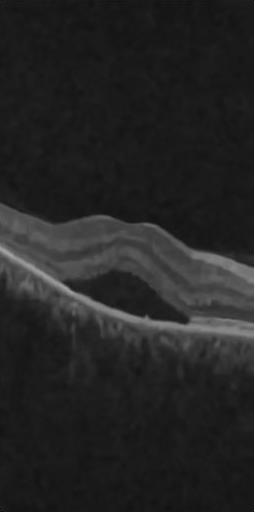
\includegraphics[width = 0.3\textwidth, height = 0.2\textheight]{figures/Denoising.jpg} % scale, width, height 
  \caption{De-noising B-scan Slice}
  \label{fig:Denoising image}
\end{figure}
\item \textbf{Flattening}: is the function used to make the layers of an image almost straight based on the function applied either fitting a polynomial or RANSAC.
SD-OCT images of the retina have a natural curvature as noticed in the figure 3.1, which is further distorted due to the common practices in OCT image acquisition and display that varies both between patients and within each SD-OCT volume.
Following Srinivasan et al. way we reduce the effects of the perceived retinal curvature when classifying SD-OCT images, we flatten the retinal curvature in each image.
To flatten the retinal curvature in each SD-OCT image:
\begin{itemize}
\item calculate a pilot estimate of the retinal pigment epithelium layer (RPE).
\item calculate the convex hull around the pilot RPE points, and use the lower border of the convex hull as an estimate of the lower boundary of the retina.
\item remove outliers by applying a [1 * 3] median filter (MATLAB notation) to this estimate.
\item Unlike Srinivasan et al. in his work for creating the flattened image, he fitted the second order polynomial to make the estimation of retinal lower boundary points.
Random Sample Consensus(RANSAC) function is applied to do the same job with better accuracy of line allignment.
An iterative method to achieve parameter estimation of a model from set of data with outliers.
With the accuracy achieved in RANSAC but there's a disadvantage of time as it has no limited time to do the job, until it finds the best alignment it will stop, otherwise it will continue calculating.
\end{itemize}
\begin{figure}[htb]
        \centering
        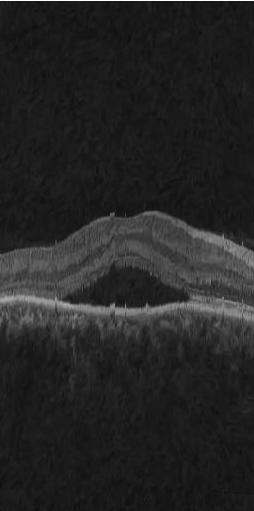
\includegraphics[width = 0.3\textwidth, height = 0.2\textheight]{figures/flattening.jpg} % scale, width, height 
  \caption{Flattening B-scan Slice}
  \label{fig:Flattening image}
\end{figure}

\item \textbf{Cropping}:this method is used to crop the region interested to save time when the data required for classification might take time.
Thus, to differentiate between the volumes with disease or not, limiting the targeted place might help the classifier to set the data clearly.
The cropping in our SERI data is bigger than the cropping region done by Srinivasan et al.
In the axial dimension, all images are cropped 325 pixels from over the RPE and 30 pixels under the RPE.
In the lateral dimension, all images are cropped 340 pixels to the center.
\begin{figure}[htb]
        \centering
        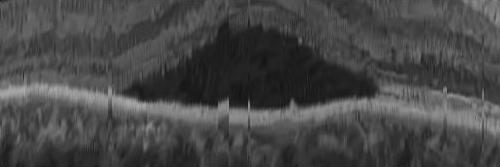
\includegraphics[width = 0.3\textwidth, height = 0.2\textheight]{figures/cropping.jpg} % scale, width, height 
  \caption{Cropping B-scan Slice}
  \label{fig:Cropping image}
\end{figure}

\end{enumerate} 

\subsection{Feature Extraction}

This part of the pipeline is meant to create informative data from measured data and build values (features), which they are non-redundant and lead to better interpretations.
It is crazy to take all features and in our case it reached up to 113215 dimension for 32 volumes, which real data is lost, only 32 points in this great number of dimensions.
It describes content of the features in images, algorithms and application and so on, 
This process finds out the connection between pixels in a particular image.
Descriptors describe the main characteristics such as shape, texture and many other aspects in image.
Descriptors are  divided into two groups:
\begin{itemize}
\item \textbf{General information descriptors}: give description of colour, shape , texture, basically low level descriptors.
\item \textbf{Specific domain information descriptors}: give description about events or objects like face recognition.
\end{itemize}

In the pipeline, implementation of Histogram of Oriented Gradients (HOG) and Local binary patterns (LBP) is applied and the explanation as follow:
\begin{enumerate}
\item \textbf{Histogram of Oriented Gradients (HOG)}: is a feature descriptor for object detection.
This descriptors are used based on gradient orientation in well-localized portion in an image.
It is computed based on overlapping local contrast normalization on a dense grid on uniform cells to enhance the accuracy.
HOG descriptors divides the image into connected cells by counting the the strength and orientation of the gradient spatial in every cell.
Basically, image is divided into small cells and 1-D histogram of the directions of the gradients is calculated for every by gradient magnitude.
To make the descriptors invariant to shadowing and different illumination, descriptor vectors blocks are normalized over larger overlapping blocks then renormalizing.
This results into a feature vector for each image with normalized histograms.

In our implementation, as Srinivasan et al. did, the extraction of HOG with [4*4] cell size, [2*2] cells per cell, a block overlap of [1*1] cells, unsigned gradients and 9 orientation histogram bins.
Extraction of HOG features at four levels of the multi-scale Gaussian low-pass pyramid to have multiple scale levels structure.
Furthermore, concatenate all HOG vectors for each image to obtain the set of histograms to be ready for the feature representation or classification.  
\item \textbf{Local binary patterns (LBP)}: is a visual descriptor and usually combined with HOG to improve the performance of detection on some dataset as our implementation did.
It starts with dividing the window of an image to cells (8*8 pixels for every cell).
After that, a comparison of each pixel with its 8, 16 and 24 neighbours.
Followed by clockwise or counter-clockwise circle along the pixels.
The decision making in this process, "0" value is assigned to the pixel if the center pixel value is greater than neighbour’s value, otherwise assign value "1".
Then, the histogram is computed over the cell by the appearing pixels frequency based on the threshold of higher or less than the center.
Normalizing the vector feature is done.
Finally, concatenating all histograms from all cells in all images to make $128$ vectors for all volume.
this data is ready to be directed for further feature representation or directly to the classifier.
\end{enumerate} 

\subsection{Feature Representation}
The great number of dimensions resulted from the previous section make the time calculation high for classification and hence it loses the main points in the dimension.
Many irrelevant feature vectors are produced, which reduces the precision and performance of system, so it is very crucial to learn the most important and uncorrelated features.
In another words, Feature representation is the way to create a new space for features either by making a new model for features or reducing the real features to more meaningful dimensions. 

There many types of feature representation methods, like Linear Discriminant Analysis (LDA), Principal Component Analysis (PCA), Sequential Forward Feature Selection (SFFS) and Sequential Backward Feature Selection (SBFS).
SFFS and SBFS is used to chose the most correlated dimensions, while PCA and LDA are projecting data into new space by reducing dimensions.
Bag of Words (BoW) is a feature representation way that try to find similar patterns based on creating dictionary or words in clusters for features in the space.
This section will explain the methods we used in the pipeline:
\begin{enumerate}
\item \textbf{Principal Component Analysis (PCA)}: is feature reduction method for the extracted data, which looks for subspaces where variation is maximized.
It is unsupervised, statistical orthogonal linear transformation approach where the subspace transformed data is relevant and uncorrelated .
The process of PCA basically, is done by picking up the highest variance value in the dimension till it reaches to the number chosen to be reduced.
The principal components are orthogonal transformation because they are the eigenvectors of the covariance matrix, which is symmetric.
PCA is sensitive to the repetitive scaling of the original variables, hence reducing the dimensions can not be achieved, a kernel of PCA is used to find subspaces.

PCA is the way of fitting some data from a lot of dimensions where each axis means a principle component.
Sometimes if the axis is small compare to others so the variance along the axis is small, hence the lose of some useful information is happened by deleting that axis. 
The math way of PCA is organized as follows
\begin{itemize}
\item subtracting the mean from each point in the dataset to gather data around origin center.
\item Calculating the covariance matrix of centred data.
\item Computing the eigenvectors covariance matrix corresponding eigenvectors.
\item Orthogonalizing eigenvectors sets then converting them to unit vectors by normalizing the eigenvectors.
\end{itemize}

In this project, reduction of HOG and LBP dimensions to 40 and 20 dimensions respectively.
The dimensions reduced are concatenated before BoW applied for creating dictionary of the data.
Mainly, the reduction was done based on Singular value decomposition (SVD), due to the accuracy produced with acceptable processing speed.
The avoidance of using Eigenvalue decomposition (EIG) cause the less accurate results generated compared to SVD, even-though it is faster.
There is another method to reduce feature data in PCA using Alternating least squares (ALS) algorithm, which can work well for data sets with a small percentage of missing data at random, but might not perform well on sparse data sets\cite{jackson2005user}.

\item \textbf{Bag of Words (BoW)}: is a clustering method for the extracted data by modelling them to a new space.
The number of repeating of pattern will make the decision how to cluster the data.
Clustering belongs to the use of k-means to make the cluster for the feature space so that k represent the number of words, histograms or samples number of minority class.
Hence, the centroids of these clusters define the new samples from the majority class.
BoW clusters are the set of low-level features using a k-means algorithm to produce a “codebook” of “visual words”.
Every visual word have a centroid that belongs to a cluster.
After generating the words, every centroid is represented by histogram based on the number of the occurrence of the words from extracted features \cite{sun2012automatic}.
K-means algorithm is an iterative method, which finds k centroids by alternating assignment and update steps.
Euclidean distance method is used for alternating assignment.
In this project, many tests involved using different number of k centroid and vary between 10-60.
The results of BoW will be shown in the next chapter.
\end{enumerate}

\subsection{Classification}
Classification is a method used to map an input data to its category.
This terminology task is to recognize the pattern after giving some data similar to it in a process called training.
Training might be attached with labels to be supervised learning or without labels to be unsupervised learning.
This part of the project is using supervised learning method with labels for Normal volumes and another label for DME volumes.
Three different classifier are used for comparison: Random Forest (RF), linear, and kernel- Support Vector Machine (SVM).
Using the feature descriptor provided the first two representations.
The classifiers are trained to classify B-scans and volume classification is performed based on the total number of diseased B-scans per volume using a majority vote rule and cross validation.
Here in this section we explain briefly about the classifiers used as follow:
\begin{enumerate}
\item \textbf{linear-Support Vector Machine (SVM)}: is a supervised learning algorithm based on training feature vectors to categorize whatever number of categories.
SVM creates set of points in space for a category then divided by a reasonable gap and make line to separate points for each category\cite{vermeer2011automated}.
The new separation of points mapped and predicted to make a decision for the classifier as shown in the SVM figure.
In this part, we used the Matlab function svmtrain but it did not converge then we used fitcsvm function with predict function to classify data.

\begin{figure}[htb]
        \centering
        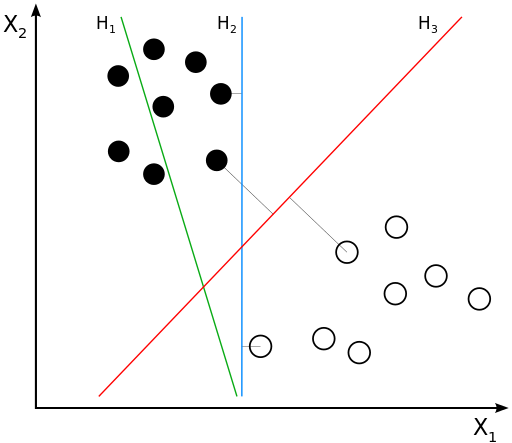
\includegraphics[width = 0.3\textwidth, height = 0.3\textheight]{figures/SVM.png} % scale, width, height 
  \caption{Linear-SVM \cite{SVMmethod}}
  \label{fig:SVM}
\end{figure}

\item \textbf{kernel-Support Vector Machine (SVM)}: is exactly the same process of linear SVM but in non-linear way to maximize-margin hyperplanes, as shown in the figure 3.7.
This classifier is changing every dot product with the non-linear kernel function.
This allows to achieve the maximize-margin hyperplanes in the feature space transformation.
The plane might not by linear from input data to be transformed as shown.
Working in a higher-dimensional feature space will increase the chances of producing the generalization error of support vector machines, although given enough samples the kernel achieve good performance.
Here fitcsvm is the Matlab function used to perform this part with kernal RBF.
\begin{figure}[htb]
        \centering
        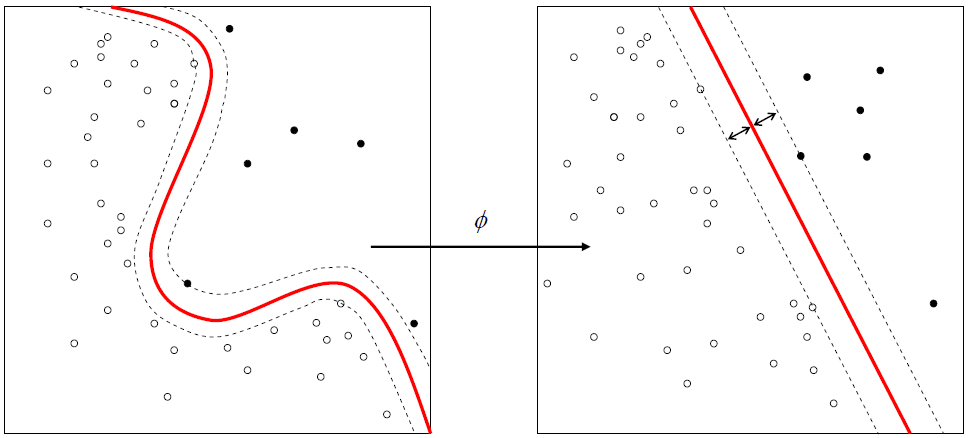
\includegraphics[width = 0.3\textwidth, height = 0.3\textheight]{figures/Kernel_Machine.png} % scale, width, height 
  \caption{Kernal-SVM \cite{SVMmethodkernal}}
  \label{fig:SVM}
\end{figure}

\item \textbf{Random Forest (RF)}: is a classifier that creates trees and then sub-tress based on the targeted number of trees wanted.
The more trees to create in this random forest the more time required to compute and the more details that process obtained.
This classifier is averaging many trees and sub-trees decision.
The average taken is trained on different features in the training set to reduce the variance.
This method uses the modified bagging algorithm, which selects random sample with replacement and fits trees into the samples, which differs from the bagging algorithm that targets to decrease the variance which will lead to better performance without even increasing the bias.
This means, increasing the number of trees will yield to correlated trees and this will increase the sensitivity to noise, hence bootstrap sampling will de-correlate the trees.

This classifier is enhancing the performance usually, but sometimes with the increasing of trees number the results might stay the same so in here \cite{oshiro2012many} proved that between 64-128 trees are performing good in term of accuracy, memory and time required.
In our project we aimed for 80 trees and results shown in next chapter. 
\end{enumerate} 
\subsection{Evaluation Of Classification}
This section briefly explains the way used to validate and evaluate the results obtained from the classifiers mentioned in the previous section.
The results were having the assessment based on:
\begin{itemize}
\item \textbf{Validation}: is the way to generalize the classification results.
In this section, we performed leave-two-patient-out-cross-validation, where we take the first voxel from DME images and first voxel from normal images out for testing and the 30 other volumes are processed for training.
After that, changing the testing set by substituting the first voxel with second voxel and so on ... 
for 16 times cause we have 32 volumes.   
\item \textbf{Evaluation}: is a method to make results shown and determines the method quality for further comparison.
A confusion matrix is done to classify the results and in our case the confusion matrix has two rows and columns, because we classified based on the volume type either diseased or normal.
\begin{figure}[htb]
        \centering
        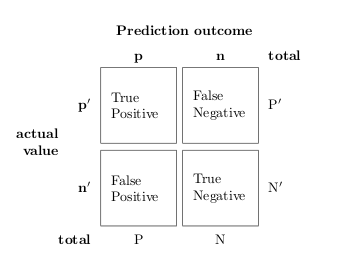
\includegraphics[width = 0.3\textwidth, height = 0.3\textheight]{figures/Confusion.png} % scale, width, height 
  \caption{Confusion Matrix for evaluation \cite{confusion}}
  \label{fig:Confusion}
\end{figure}

The figure shows the evaluation way followed in this project as the True positive (TP) and true negative (TN) are the samples that are correctly predicted to belong to the disease or normal class, respectively.
False positive (FP) and false negative (FN) are predicted as the FP in the negative class while it is in the positive class and vice versa.
The confusion matrix is the famous method to compute the accuracy (ACC), sensitivity (SE), specificity (SP), and precision.
The equations to calculate the accuracy, sensitivity are shown in equation 3.1 and 3.2 respectively.
Another aspects used to evaluate the method performance like F-score and Percision.
\begin{equation}
Sensitivity = \frac{TP}{TP+FN}
\end{equation}
and,

\begin{equation}
Specificity = \frac{TN}{TN+FP}
\end{equation} 
and,

\begin{equation}
Percision = \frac{TP}{TP+FP}
\end{equation}
\end{itemize}

\section{Automatic Segmentation Of OCT Volumes}
Inspired by deep learning methods to learn very deeply the details of an image or certain patteren for better classification or knoweldge for the machine wanted to learn the task.
This section is explaining the method used to segment the OPTIMA challenge data as shown in figure 3.9.
The rest of the section present into details each intermediate step.
In \cite{venhuizen2015autCNN}, the method propsed using neural network using CNN method to segment his data, while the segmentation in this part was done using autoencoder.
This method based on extracting Maximally stable extremal regions (MSER) with specific threshold and then cropping each reigon.
After that, comparing the cropped images with the images resulted from Simultaneous truth and performance level estimation (STAPLE) for label validation.
Assigning the patches with labels to auto-encoder for learning and feature extraction, then classification followed by comparing the testing data with the network built in the autoencoder to validate the results in confusion matrix.

\begin{figure}[htb]
        \centering
        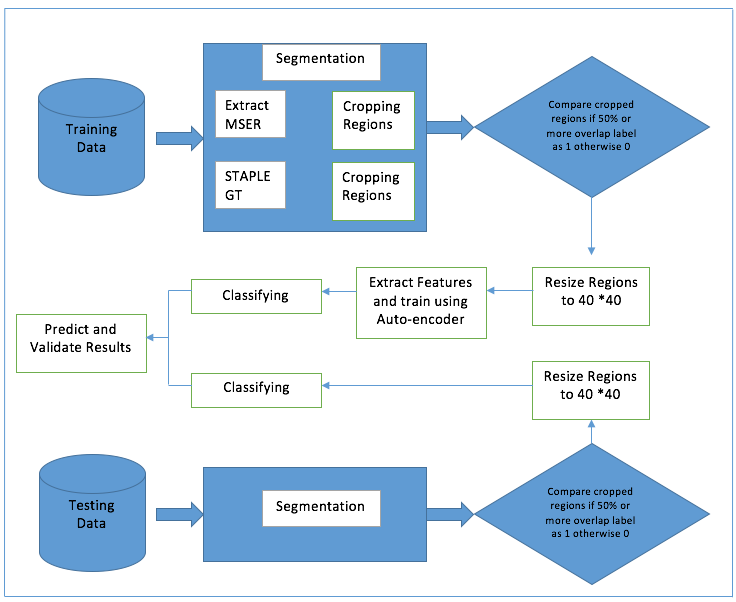
\includegraphics[width = 0.9\textwidth, height = 0.5\textheight]{figures/Segmentation.png} % scale, width, height 
  \caption{Segmentation Pipeline}
  \label{fig:Segmentation Pipeline}
\end{figure} 
\subsubsection{Segmentation Process}
This section explains the steps used to segment an image as many researchers proposed many methods as shown in chapter 2.2.2. and as follow:
\begin{enumerate}
\item\textbf{Maximally stable extremal regions (MSER)}: is a method used as blob detection in images.
This algorithm proposed by Matas \cite{matas2004robust} to find correspondences between image elements and create stable regions or images inside each image.
This brialliant method led to better matching and recognition of certain regions with a very fast speed of extracting each image and to compare it with other regions in other images and has the following steps to extract regions:
\begin{itemize}
\item Sorting pixels by intensity.
\item Marking the set of pixels of each region in different color and the list of merging connected components using union-find algorithm.
\item Data structure is produced as a function of intensity of connected pixels.
\item two components are merged into larger region if the two groups are smaller than the threshold value set to form one region.
\item Regions presented are the the results of the stable regions over large range of threshold.
\end{itemize}
This part in our algorithm we extracted MSER regions in all images in the training and teasting data.

\item\textbf{Simultaneous truth and performance level estimation (STAPLE)}: is a method used for the validation of segmenting image.
The challenge of having optimal method to segment an image is still under research due to the differences in images and resolution.
Evaluating the performance of certain algorithm in image segmentation is a difficult process.
The reason behind that is back to different opinions of raters or experts in deciding how to make ground-truth suiting an image condition, hence the existence of STAPLE to form one ground-truth of all ground-truth presented for one image.

STAPLE is removing the variability introduced by raters to ensure the quality of the proposed method to segment.
This method is considering a collection of pixels representing the segmentation and then computing the probabilistic estimate of the true segmentation.
The probabilistic estimate of the true segmentation is achieved by predicting the optimal combination of the raters segmentation, weighting each segmentation based on the estimated performance level.
Then, incorporating a prior model for the spatial distribution of structures being segmented, as well as spatial homogeneity constraints.
STAPLE is a stright method to use and apply in clinical imaging data, it can enable assessment of the performance of an automated image segmentation algorithm, and enables direct comparison of human rater and algorithm performance\cite{warfield2004simultaneous}.
OPTIMA data includes two ground truths and using STAPLE to validate the two ground truths to produce one ground truth used later for comparision explained next.
\item\textbf{Comparing Patches}:is a process to compare regions extracted from MSER with regions extracted from STAPLE ground truth and then resizing the regions to fit it to the auto-encoder.
\end{enumerate}

\subsection{Autoencoder Training And Feature Extraction}
Autoencoder is neural network which is copying the inputs to its outputs in the training process.
It has different hidden layes internally that represent the input data.
The network has two parts which are anencoder function $h=f(x)$ and decoder which generate the reconstruction $r=g(h)$.
Usually auto-encoders are restricted in ways that allow them to learn to copy only input that feeds the training data.
Because the model is forced to prioritize, which aspects of the input should be copied, it often learns useful properties of the data and the structure of auto-encoder as shown in figure 3.10.
Typically, auto-encoders used for reducing the dimensions or feature extraction.

\begin{figure}[htb]
        \centering
        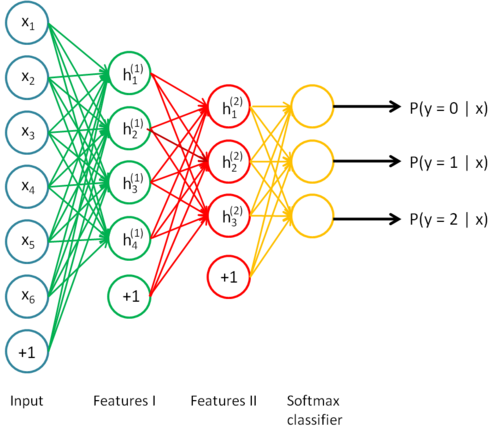
\includegraphics[width = 0.9\textwidth, height = 0.5\textheight]{figures/Autoencoder.png} % scale, width, height 
  \caption{Autoencoder Layout}
  \label{fig:Autoencoder Layout}
\end{figure} 

Auto-encoder is used for training and the algorithm can be summed up as:
\begin{itemize}
\item Feed-forward each input $x$ to calculate the activations in all hidden layers and at the output layers to obtain $x'$.
\item Using squared error, measure the deviation of $x'$ from the input $x$.
\item Backpropagate the error and update the new weight in the net.  
\end{itemize}

Auto-encoder is trained using backpropagation (Fine tuning), which calculates the gradient of the loss function with respect to weights through the network.
This gradient is used to optimize the algorithm, which is used later to update the weights to minimize the loss function\cite{liou2014autoencoder}.
Backpropagation demand a known output for each input to compute the loss function gradient. 
This method is supervised and it is used in unsupervised method in auto-encoder.
Using backpropagation to train network with many hidden layers will make the first layer when it recieved the error insignificant, hence conjugate gradient method can solve this problem.
Another way to solve this slow process by setting intial weights that estimate the final output.
In this project, we train the autoencoder with 100 hidden layers at the first hidden layer then 50 hidden layers at the second layer. then it is classified using softmax layer classifier.

\subsection{Classification} is the process of spotting the differences between various classes.
This process is explained in 3.2.4. 
In this part, SVM. or SVM-RBF or RF are not used, but Softmax layer is used instead for classifying the existence of the cyst or not.
Softmax layer is a generalization of the logistic function which is implemented at the last layer of the network.
\subsection{Evaluation And Validation} this process is evaluated using the confusion Matrix.
Validation of the results was done based on the same aspects as in section 3.2.5 which they are Percision, Sensitivity and Accuracy.

 














\chapter{Results And Discussion} \label{chap:results}

This section presents the results and the discussion of all experiments.
Presenting the results based on validation and evaluation process mentioned in the previous chapter.
We have divided this section into two parts, which is based on classifying images in the first part and classifying potential regions inside the image for the second part.
Inside each section, some subsections presenting the results for each section.
In classification section, SERI data is used, and OPTIMA challenge data is used in the second section.

\section{Classification Experiments}
\subsection{Experiments}
This section presents the results obtained from different classifiers like linear-SVM, SVM-RBF and RF respectively.
First, the 32 volumes are loaded, then two of them are excluded for testing and 30 for training, hence this process is performed 16 times to validate the results based on cross validation.
Then, each B-scan image is de-noised using sparsity-based block matching and 3D-filtering (BM3D), which is available online with a harded-threshold , and then flattened the image.
Flattening is done by computing the RPE layer, then we compute the convex hull around RPE points and using the lower line of the retina, then applying median filter to remove any outliers.
This almost flatten image is then applied to RANSAC to make lines straight.
After that, we cropped the targeted location, which consists the disease usual place for having accurate classification and to avoid any not important details.

Instead of dividing images into patches, we extract HOG and LBP at four different scale levels using impyarmid then concatenate them into one single vector for each image.
After that, for some parts of the test as shown in the tables below, the feature vectors are concatenated from all volumes and sent directly to the classifiers.
Some other cases are representing the features in before sending them to the classifier.
Since the great number of dimensions produced from HOG or LBP (rotation invariant (–ri) and non- rotation invariant (–nri) LBP features with various radius, {8,16,24})or both which are almost 116235 vectors, PCA is used to reduce the dimensions for both discriptors 40 dimensions for HOG and 20 for LBP such that the most discriminative components are kept.
Some of experiments sending the PCA of HOG to classifiers directly or lbp or concatenating bot and send them to classifiers.

Another way to represent the feature vectors by creating dictionaries or words then converting the words to histograms based on kmeans and send them to the classifiers and the optimal number of words has been selected heuristicallyas as shown in table 4.4.
And finally the classifiers shown the results in table 4.1,4.2,4.3 and 4.4 based on confusion matrix of cross validation.
\begin{table*}
\caption{Experiments based Linear-SVM.}
\centering
\resizebox{1\textwidth}{!}{
\begin{tabular}{l ccccc}
  \toprule 
  Features & \multicolumn{5}{c}{Evaluation}\\
  \cmidrule{2-6}  
  & Sensitivity & Specificity & Precision & F1-score & Accuracy \\
  \midrule
  \multicolumn{6}{c}{}\\[-1.5ex]
  \acs{hog} & 0.69 & 0.94 & 0.91 & 0.81 & 0.78 \\
  \multicolumn{6}{c}{}\\[-1.5ex]

  \acs{hog}$^{\acs{pca}}$ & 0.75 & 0.87 & 0.85 & 0.80 & 0.81\\
  \multicolumn{6}{c}{}\\[-1.5ex]
 
  \acs{lbp}$_{8-ri}$ & 0.63 & 0.81 & 0.77 & 0.69 & 0.72\\
  \multicolumn{6}{c}{}\\[-1.5ex] 

  \acs{lbp}$_{8-ri}^{\acs{pca}}$ & 0.88 & 0.88 & 0.88 & 0.88 & 0.88\\
  \multicolumn{6}{c}{}\\[-1.5ex]   

  \acs{lbp}$_{8-nri}$ & 0.63 & 0.81 & 0.79 & 0.73 & 0.75\\
  \multicolumn{6}{c}{}\\[-1.5ex] 

  \acs{lbp}$_{8-nri}^{\acs{pca}}$ & 0.63 & 0.88 & 0.83 & 0.71 & 0.75\\
  \multicolumn{6}{c}{}\\[-1.5ex]

  \acs{lbp}$_{16-ri}$ & 0.75 & 0.75 & 0.75 & 0.75 & 0.75\\
  \multicolumn{6}{c}{}\\[-1.5ex] 

  \acs{lbp}$_{16-ri}^{\acs{pca}}$ & 0.75 & 0.75 & 0.75 & 0.75 & 0.75\\
  \multicolumn{6}{c}{}\\[-1.5ex]  

  \acs{lbp}$_{16-nri}$ & 0.69 & 0.81 & 0.79 & 0.73 & 0.75\\
  \multicolumn{6}{c}{}\\[-1.5ex] 

  \acs{lbp}$_{16-nri}^{\acs{pca}}$ & 0.63 & 0.88 & 0.83 & 0.71 & 0.75\\
  \multicolumn{6}{c}{}\\[-1.5ex]   

  \acs{lbp}$_{24-ri}$ & 0.69 & 0.88 & 0.85 & 0.76 & 0.78\\
  \multicolumn{6}{c}{}\\[-1.5ex] 
 
  \acs{lbp}$_{24-ri}^{\acs{pca}}$ & 0.81 & 0.81 & 0.81 & 0.81 & 0.81\\
  \multicolumn{6}{c}{}\\[-1.5ex]  

  \acs{lbp}$_{24-nri}$ & 0.69 & 0.88 & 0.85 & 0.76 & 0.78\\
  \multicolumn{6}{c}{}\\[-1.5ex] 

  \acs{lbp}$_{24-nri}^{\acs{pca}}$ & 0.69 & 0.88 & 0.85 & 0.76 & 0.78\\
  \multicolumn{6}{c}{}\\[-1.5ex]     

   \acs{hog}$^{\acs{pca}}$ +\acs{lbp}$_{8-ri}^{\acs{pca}}$ & 0.69 & 0.81 & 0.79 & 0.73 & 0.75\\
  \multicolumn{6}{c}{}\\[-1.5ex]
  
   \acs{hog}$^{\acs{pca}}$ +\acs{lbp}$_{16-ri}^{\acs{pca}}$ & 0.75 & 0.88 & 0.86 & 0.8 & 0.81\\
  \multicolumn{6}{c}{}\\[-1.5ex]
  
   \acs{hog}$^{\acs{pca}}$ +\acs{lbp}$_{24-ri}^{\acs{pca}}$ & 0.69 & 0.88 & 0.85 & 0.79 & 0.78\\
  \multicolumn{6}{c}{}\\[-1.5ex]

 \acs{hog}$^{\acs{pca}}$ +\acs{lbp}$_{8-nri}^{\acs{pca}}$ & 0.69 & 0.75 & 0.73 & 0.71 & 0.72\\
  \multicolumn{6}{c}{}\\[-1.5ex]
  
  \acs{hog}$^{\acs{pca}}$+\acs{lbp}$_{8-nri}^{\acs{pca}}$+\acs{lbp}$_{16-nri}^{\acs{pca}}$+\acs{lbp}$_{24-nri}^{\acs{pca}}$ & 0.62 & 0.75 & 0.71 & 0.66 & 0.68 \\
  \multicolumn{6}{c}{}\\[-1.5ex]

  \acs{hog}$^{\acs{pca}}$+\acs{lbp}$_{8-ri}^{\acs{pca}}$+\acs{lbp}$_{16-ri}^{\acs{pca}}$+\acs{lbp}$_{24-ri}^{\acs{pca}}$ & 0.69 & 0.81 & 0.78 & 0.73 & 0.75 \\
  \multicolumn{6}{c}{}\\[-1.5ex]
 
\bottomrule
\end{tabular}}
\end{table*}


\begin{table*}
\caption{Experiments based Linear-SVM-RBF.}
\centering
\resizebox{0.85\textwidth}{!}{
\begin{tabular}{l ccccc}
  \toprule 
  Features & \multicolumn{5}{c}{Evaluation}\\
  \cmidrule{2-6}  
  & Sensitivity & Specificity & Precision & F1-score & Accuracy \\
  \midrule
  \multicolumn{6}{c}{}\\[-1.5ex]
  \acs{hog} & 0.94 & 0.06 & 0.50 & 0.65 & 0.50 \\
  \multicolumn{6}{c}{}\\[-1.5ex]

  \acs{hog}$^{\acs{pca}}$ & 0.13 & 0.88 & 0.50 & 0.20 & 0.50\\
  \multicolumn{6}{c}{}\\[-1.5ex]

  \acs{lbp}$_{8-ri}$ & 0.94 & 0.25 & 0.55 & 0.70 & 0.59\\
  \multicolumn{6}{c}{}\\[-1.5ex] 

  \acs{lbp}$_{8-ri}^{\acs{pca}}$ & 0.81 & 0.81 & 0.81 & 0.81 & 0.81\\
  \multicolumn{6}{c}{}\\[-1.5ex]   

  \acs{lbp}$_{8-nri}$ & 1.00& 0.00 & 0.50 & 0.67 & 0.50\\
  \multicolumn{6}{c}{}\\[-1.5ex] 

  \acs{lbp}$_{8-nri}^{\acs{pca}}$ & 0.81 & 0.31 & 0.54 & 0.65 & 0.56\\
  \multicolumn{6}{c}{}\\[-1.5ex]

  \acs{lbp}$_{16-ri}$ & 0.88 & 0.25 & 0.54 & 0.67 & 0.56\\
  \multicolumn{6}{c}{}\\[-1.5ex] 
 
  \acs{lbp}$_{16-ri}^{\acs{pca}}$ & 0.81 & 0.88 & 0.87 & 0.84 & 0.84\\
  \multicolumn{6}{c}{}\\[-1.5ex]  
 
  \acs{lbp}$_{16-nri}$ & 1.00 & 0.00 & 0.50 & 0.67 & 0.50\\
  \multicolumn{6}{c}{}\\[-1.5ex] 

  \acs{lbp}$_{16-nri}^{\acs{pca}}$ & 0.81 & 0.50 & 0.62 & 0.70 & 0.66\\
  \multicolumn{6}{c}{}\\[-1.5ex]   

  \acs{lbp}$_{24-ri}$ & 0.88 & 0.50 & 0.64 & 0.74 & 0.69\\
  \multicolumn{6}{c}{}\\[-1.5ex] 

  \acs{lbp}$_{24-ri}^{\acs{pca}}$ & 0.75 & 0.88 & 0.86 & 0.80 & 0.81\\
  \multicolumn{6}{c}{}\\[-1.5ex]  
 
  \acs{lbp}$_{24-nri}$ & 1.00 & 0.00 & 0.50 & 0.67 & 0.50\\
  \multicolumn{6}{c}{}\\[-1.5ex] 

  \acs{lbp}$_{24-nri}^{\acs{pca}}$ & 0.69 & 0.81 & 0.79 & 0.73 & 0.75\\
  \multicolumn{6}{c}{}\\[-1.5ex] 
  
   \acs{hog}$^{\acs{pca}}$ +\acs{lbp}$_{8-ri}^{\acs{pca}}$ & 0.69 & 0.81 & 0.79 & 0.73 & 0.75\\
  \multicolumn{6}{c}{}\\[-1.5ex]

   \acs{hog}$^{\acs{pca}}$ +\acs{lbp}$_{8-nri}^{\acs{pca}}$ & 0.00 & 1.00 & NAN & 0.00 & 0.50\\
  \multicolumn{6}{c}{}\\[-1.5ex]

   \acs{hog}$^{\acs{pca}}$ +\acs{lbp}$_{16-ri}^{\acs{pca}}$ & 0.19 & 0.94 & 0.75 & 0.30 & 0.56\\
  \multicolumn{6}{c}{}\\[-1.5ex]

  \acs{hog}$^{\acs{pca}}$ +\acs{lbp}$_{16-nri}^{\acs{pca}}$ & 0.63 & 0.94 & 0.50 & 0.11 & 0.50\\
  \multicolumn{6}{c}{}\\[-1.5ex]

 \acs{hog}$^{\acs{pca}}$ +\acs{lbp}$_{24-ri}^{\acs{pca}}$ & 0.00 & 1.00 & NAN & 0.00 & 0.50\\
  \multicolumn{6}{c}{}\\[-1.5ex]

  \acs{hog}$^{\acs{pca}}$ +\acs{lbp}$_{24-nri}^{\acs{pca}}$ & 0.13 & 0.94 & 0.67 & 0.21 & 0.53\\
  \multicolumn{6}{c}{}\\[-1.5ex]
 
\bottomrule
\end{tabular}}
\end{table*}


\begin{table*}
\caption{Experiments based Random Forest.}
\centering
\resizebox{0.85\textwidth}{!}{
\begin{tabular}{l ccccc}
  \toprule 
  Features & \multicolumn{5}{c}{Evaluation}\\
  \cmidrule{2-6}  
  & Sensitivity & Specificity & Precision & F1-score & Accuracy \\
  \midrule
  \multicolumn{6}{c}{}\\[-1.5ex]
  \acs{hog} & 0.63 & 1.00 & 1.00 & 0.77 & 0.81 \\
  \multicolumn{6}{c}{}\\[-1.5ex]

  \acs{hog}$^{\acs{pca}}$ & 0.56 & 0.94 & 0.90 & 0.69 & 0.75\\
  \multicolumn{6}{c}{}\\[-1.5ex]

  \acs{lbp}$_{8-ri}$ & 0.75 & 0.81 & 0.80 & 0.74 & 0.78\\
  \multicolumn{6}{c}{}\\[-1.5ex] 

  \acs{lbp}$_{8-ri}^{\acs{pca}}$ & 0.75 & 0.81 & 0.80 & 0.74 & 0.78\\
  \multicolumn{6}{c}{}\\[-1.5ex]   

  \acs{lbp}$_{8-nri}$ & 0.69 & 0.81 & 0.79 & 0.73 & 0.75\\
  \multicolumn{6}{c}{}\\[-1.5ex] 

  \acs{lbp}$_{8-nri}^{\acs{pca}}$ & 0.75 & 0.81 & 0.80 & 0.77 & 0.78\\
  \multicolumn{6}{c}{}\\[-1.5ex]

  \acs{lbp}$_{16-ri}$ & 0.81 & 0.88 & 0.87 & 0.84 & 0.84\\
  \multicolumn{6}{c}{}\\[-1.5ex] 

  \acs{lbp}$_{16-ri}^{\acs{pca}}$ & 0.75 & 0.94 & 0.92 & 0.83 & 0.84\\
  \multicolumn{6}{c}{}\\[-1.5ex]  

  \acs{lbp}$_{16-nri}$ & 0.69 & 1.00 & 1.00 & 0.81 & 0.84\\
  \multicolumn{6}{c}{}\\[-1.5ex] 

  \acs{lbp}$_{16-nri}^{\acs{pca}}$ & 0.75 & 0.88 & 0.86 & 0.80 & 0.81\\
  \multicolumn{6}{c}{}\\[-1.5ex]   

  \acs{lbp}$_{24-ri}$ & 0.69 & 0.94 & 0.92 & 0.79 & 0.81\\
  \multicolumn{6}{c}{}\\[-1.5ex] 

  \acs{lbp}$_{24-ri}^{\acs{pca}}$ &  0.75 & 0.94 & 0.92 & 0.83 & 0.84\\
  \multicolumn{6}{c}{}\\[-1.5ex]  

  \acs{lbp}$_{24-nri}$ & 0.69 & 0.94 & 0.92 & 0.79 & 0.81\\
  \multicolumn{6}{c}{}\\[-1.5ex] 

  \acs{lbp}$_{24-nri}^{\acs{pca}}$ & 0.75 & 0.88 & 0.86 & 0.80 & 0.81\\
  \multicolumn{6}{c}{}\\[-1.5ex]       
  
   \acs{hog}$^{\acs{pca}}$ +\acs{lbp}$_{8-ri}^{\acs{pca}}$ & 0.63 & 0.81 & 0.77 & 0.69 & 0.72\\
  \multicolumn{6}{c}{}\\[-1.5ex]

   \acs{hog}$^{\acs{pca}}$ +\acs{lbp}$_{8-nri}^{\acs{pca}}$ & 0.63 & 0.81 & 0.77 & 0.69 & 0.72\\
  \multicolumn{6}{c}{}\\[-1.5ex]

   \acs{hog}$^{\acs{pca}}$ +\acs{lbp}$_{16-ri}^{\acs{pca}}$ & 0.75 & 0.88 & 0.86 & 0.80 & 0.81\\
  \multicolumn{6}{c}{}\\[-1.5ex]

  \acs{hog}$^{\acs{pca}}$ +\acs{lbp}$_{16-nri}^{\acs{pca}}$ & 0.63 & 0.88 & 0.83 & 0.71 & 0.75\\
  \multicolumn{6}{c}{}\\[-1.5ex]

 \acs{hog}$^{\acs{pca}}$ +\acs{lbp}$_{24-ri}^{\acs{pca}}$ & 0.63 & 0.88 & 0.83 & 0.71 & 0.75\\
  \multicolumn{6}{c}{}\\[-1.5ex]

  \acs{hog}$^{\acs{pca}}$ +\acs{lbp}$_{24-nri}^{\acs{pca}}$ & 0.69 & 0.88 & 0.85 & 0.76 & 0.78\\
  \multicolumn{6}{c}{}\\[-1.5ex]

\bottomrule
\end{tabular}}
\end{table*}

\begin{table}
\caption{ Classification results using Histogram+\ac{pca}+\ac{bow} representation.}
\centering
\resizebox{0.60\textwidth}{!}{
\begin{tabular}{l c c  lcr}
 \toprule
 \multicolumn{6}{c}{Histogram + \acs{pca} + \acs{bow}}\\
 \midrule
 &  &  & \multicolumn{3}{c}{Metric}  \\
 \cmidrule{4-6}
 & Classifier & \# Words & \acs{se} & \acs{sp} & \acs{pre} \\
 \midrule  
 \acs{hog}$^{\acs{pca}}$ +\acs{lbp}$_{8-ri}^{~PCA}$ & Linear-\acs{svm} & 10 & 0.38 & 0.69 & 0.55 \\
 \multicolumn{6}{c}{}\\[-1.5ex]
 
 \acs{hog}$^{\acs{pca}}$ +\acs{lbp}$_{8-ri}^{~PCA}$ & Linear-\acs{svm} & 20 & 0.31 & 0.88 & 0.71 \\
 \multicolumn{6}{c}{}\\[-1.5ex]

 \acs{hog}$^{\acs{pca}}$ +\acs{lbp}$_{8-ri}^{~PCA}$ & Linear-\acs{svm} & 30 & 0.31 & 0.94 & 0.83 \\
 \multicolumn{6}{c}{}\\[-1.5ex]
 
 \acs{hog}$^{\acs{pca}}$ +\acs{lbp}$_{8-ri}^{~PCA}$ & Linear-\acs{svm} & 40 & 0.19 & 0.94 & 0.75 \\
 \multicolumn{6}{c}{}\\[-1.5ex]

 \acs{hog}$^{\acs{pca}}$ +\acs{lbp}$_{8-ri}^{~PCA}$ & Linear-\acs{svm} & 50 & 0.38 & 0.81 & 0.67 \\
 \multicolumn{6}{c}{}\\[-1.5ex]

 \acs{hog}$^{\acs{pca}}$ +\acs{lbp}$_{8-ri}^{~PCA}$ & Linear-\acs{svm} & 60 & 0.13 & 0.88 & 0.50 \\
 \multicolumn{6}{c}{}\\[-1.5ex]

 \acs{lbp}$_{8-ri}^{~PCA}$ & Linear-\acs{svm} & 10 & 0.63 & 0.75 & 0.71 \\
 \multicolumn{6}{c}{}\\[-1.5ex]
 
 \acs{lbp}$_{8-ri}^{~PCA}$ & Linear-\acs{svm} & 20 & 0.75 & 0.38 & 0.55 \\
 \multicolumn{6}{c}{}\\[-1.5ex]

 \acs{lbp}$_{8-ri}^{~PCA}$ & Linear-\acs{svm} & 30 & 0.44 & 0.44 & 0.44 \\
 \multicolumn{6}{c}{}\\[-1.5ex]
 
 \acs{lbp}$_{8-ri}^{~PCA}$ & Linear-\acs{svm} & 40 & 0.69 & 0.56 & 0.61 \\
 \multicolumn{6}{c}{}\\[-1.5ex]

 \acs{lbp}$_{8-ri}^{~PCA}$ & Linear-\acs{svm} & 50 & 0.50 & 0.50 & 0.50 \\
 \multicolumn{6}{c}{}\\[-1.5ex]

 \acs{lbp}$_{8-ri}^{~PCA}$ & Linear-\acs{svm} & 60 & 0.69 & 0.31 & 0.50 \\
 \multicolumn{6}{c}{}\\[-1.5ex]

 \acs{lbp}$_{16-ri}$ & \acs{rbf}-\acs{svm} & 10 & 0.56 & 0.50 & 0.53 \\
 \multicolumn{6}{c}{}\\[-1.5ex]

 \acs{lbp}$_{16-ri}$ & \acs{rbf}-\acs{svm} & 20 & 0.56 & 0.63 & 0.60 \\
 \multicolumn{6}{c}{}\\[-1.5ex]
  
 \acs{lbp}$_{16-ri}$ & \acs{rbf}-\acs{svm} & 30 & 0.56 & 0.63 & 0.60 \\
 \multicolumn{6}{c}{}\\[-1.5ex]

 \acs{lbp}$_{16-ri}$ & \acs{rbf}-\acs{svm} & 40 & 0.69 & 0.56 & 0.61 \\
 \multicolumn{6}{c}{}\\[-1.5ex]

 \acs{lbp}$_{16-ri}$ & \acs{rbf}-\acs{svm} & 50 & 0.50 & 0.50 & 0.50 \\
 \multicolumn{6}{c}{}\\[-1.5ex]

 \acs{lbp}$_{16-ri}$ & \acs{rbf}-\acs{svm} & 60 & 0.75 & 0.38 & 0.55 \\
 \multicolumn{6}{c}{}\\[-1.5ex]

 \acs{lbp}$_{16-ri}$ & \acs{rf} & 10 & 0.38 & 0.63 & 0.50 \\
 \multicolumn{6}{c}{}\\[-1.5ex] 

 \acs{lbp}$_{16-ri}$ & \acs{rf} & 20 & 0.50 & 0.50 & 0.50 \\
 \multicolumn{6}{c}{}\\[-1.5ex] 

 \acs{lbp}$_{16-ri}$ & \acs{rf} & 30 & 0.44 & 0.63 & 0.54 \\
 \multicolumn{6}{c}{}\\[-1.5ex]

 \acs{lbp}$_{16-ri}$ & \acs{rf} & 40 & 0.56 & 0.50 & 0.53 \\
 \multicolumn{6}{c}{}\\[-1.5ex]

 \acs{lbp}$_{16-ri}$ & \acs{rf} & 50 & 0.38 & 0.31 & 0.35 \\
 \multicolumn{6}{c}{}\\[-1.5ex]


 \acs{lbp}$_{16-ri}$ & \acs{rf} & 60 & 0.44 & 0.38 & 0.41 \\
 \multicolumn{6}{c}{}\\[-1.5ex]

\acs{lbp}$_{16-ri}^{~PCA}$ & \acs{rf} & 10 & 0.69 & 0.38 & 0.52  \\
 \multicolumn{5}{c}{}\\[-2ex]

\acs{lbp}$_{16-ri}^{~PCA}$ & \acs{rf} & 20 & 0.56 & 0.75 & 0.69  \\
 \multicolumn{5}{c}{}\\[-2ex]

\acs{lbp}$_{16-ri}^{~PCA}$ & \acs{rf} & 30 & 0.56 & 0.38 & 0.47  \\
 \multicolumn{5}{c}{}\\[-2ex]

\acs{lbp}$_{16-ri}^{~PCA}$ & \acs{rf} & 40 & 0.50 & 0.63 & 0.57  \\
 \multicolumn{5}{c}{}\\[-2ex]
 
 \acs{lbp}$_{16-ri}^{~PCA}$ & \acs{rf} & 50 & 0.69 & 0.50 & 0.58  \\
 \multicolumn{5}{c}{}\\[-2ex]

 \acs{lbp}$_{16-ri}^{~PCA}$ & \acs{rf} & 60 & 0.56 & 0.63 & 0.60  \\
 \multicolumn{5}{c}{}\\[-2ex]

\bottomrule
\end{tabular}
}
\label{tab:tab3}
\end{table}

\subsection{Discussion}
Table 4.1 showed the results of linear-SVM classifier, and the best results was recorded for PCA either for HOG with 0.75 for sensitivity and 0.78 for specificity or LBP 0.88 for both sensitivity and specificity and when mixing both it gave lower results. 
Table 4.2 showed the lowest results when using the kernel of SVM and some of the experiments did not converge and that in the cases of mixing HOG with LBP.
Tabel 4.3 showed the best results and stable classifier using Random Forest and best results were for LBP , and this showed how LBP discriptors performed better in this project.
Finally in table 4.4 we picked up the highest results from the previous tables and performed BoW and the results were unexpected as this method shall improve the performance.
The results shown was degraded as the image was not divided into patches but it was extracting features directly to the image.

Evaluation of individual features from all tables show that the dimensionality reduction of the features improve the results of B- scan classification.
PCA is enhancing the results because it deletes the correlated dimensions and gives limited number of dimensions to make the testing and this will prove the quality of the algorithm made.
In addition, comparing individual features, LBP proves to be more discriminative than HoG features as LBP results are giving the best results and this can be explained as HOG is edge detection method and LBP is intensity detection method and SERI data classification depends on intensity to classify the disease.
Using only Histogram representation, RF classifier leads to the best performance followed by linear- SVM. RBF-SVM classifier has the lowest performance and over-fits for all the individual features while its performance improves when the number of dimensions are reduced using PCA.
Based on Tables results, the combination of LBP and HoG features does not improve the results and decreases the performance of individual features.
In this test, RF and linear-SVM have similar performance while RBF-SVM overfits.

To conclude with Exp1, tables 4.1,4.2 and 4.3 are producing the highest classification performance in this: LBP-PCA and linear-SVM, LBP-PCA and RBF-SVM, LBP16–ri and RF, and LBP16–ri with RF classifier.
These configurations are later tested in  using BoW representation. The results obtained from this experiment show that Histogram+PCA+BoW representation decreases the results.
In fact, this approach represents each volume in terms of visual-B-scans rather than visual-patches or visual-subvolumes, which could be a reason why BoW fails.
The results obtained are compared with different methods applied by other researchers into SERI data as shown in table 4.5\cite{JoanMassich2016}.
\begin{table*}
\caption{Summary of the classification performance in terms of se and sp in(\%)}
\centering
\resizebox{0.4\textwidth}{!}{
\begin{tabular}{l ccccc}
  \toprule 
   & \multicolumn{5}{c}{Evaluation}\\
  \cmidrule{2-6}  
  & Sensitivity & Specificity \\
  \midrule
  \multicolumn{6}{c}{}\\[-1.5ex]
  Lema\^itre~\textit{et~al.}~\cite{lemaitre2015classification} & 87.5 & 75.0\\
  \multicolumn{6}{c}{}\\[-1.5ex]

  Alsaih~\textit{et~al.}~\cite{alsaih2016classification}\cite{alsaih2016classification2} & 87.5 & 87.5\\
  \multicolumn{6}{c}{}\\[-1.5ex]
 
  Srinivansan~\textit{et~al.}~\cite{srinivasan2014fully} & 68.8 & 93.8\\
  \multicolumn{6}{c}{}\\[-1.5ex] 

  Venhuizen~\textit{et~al.}~\cite{venhuizen2015automated} & 61.5 & 58.8\\
  \multicolumn{6}{c}{}\\[-1.5ex]   

  Sankar~\textit{et~al.}~\cite{sankar2016classification} & 81.3 & 62.5\\
  \multicolumn{6}{c}{}\\[-1.5ex] 
  Liu~\textit{et~al.}~\cite{liu2011automated} & 68.8 & 93.8\\
  \multicolumn{6}{c}{}\\[-1.5ex] 

\bottomrule
\end{tabular}}
\end{table*}

\section{Segmentation Experiments}
\subsection{Experiments}
This section explains the results generated by auto-encoder and softmax layer classifier.
This experiment starts by extracting the MSER regions from each image and roughly there are 50-200 regions are extracted.
The MSER is extracted to cover almost all cysts appeared in an image.
Meanwhile, the STAPLE algorithm is applied to the two-ground-truths to make one reference to test the quality of the algorithm built for segmenting the B-scan images to find the cysts.
Based on STAPLE, mask is created full of zeros with equal size of B-scan images and only ones are assigned to the STAPLE ground-truth values. 
After that, images are cropped around the regions extracted by MSER and with the same cropped images size in B-scan images, mask is cropped.

To label the regions, a method is used based on the number of pixels appearing in the mask cropped images and the threshold of the sum of pixels is decided based on the average of pixels appearing and then tried many thresholds and the results shown in table 4.6.
This labelling decision is applied to both sets, training and testing data.
The training data after cropping and labelling, each cropped image is resized to 40*40 to fit into autoencoder.

As auto-encoder accepts only exact size of images to be trained.
Auto-encoder trained two hidden layers with 100 and 50 hidden layers for first and second hidden layer respectively.
After that, patches output of second autoencoder is classified using softmax layer.
With the full deep network formed as a stacked network, test images are reshaped into a matrix by changing the columns into vectors then forming the matrix.
Then, assign the test data to the network \'deepnet\'to evaluate the test patches, then compare the results obtained from the network with the actual label and analyse the results.  
To enhance the results, fine tuning (back-propagation)is applied on the whole multi-layer network.
To do this, training data shall be reshaped into vectors then concatenate them to form one matrix, like the testing data.
Finally, results are validated using confusion matrix and evaluated based on sensitivity, specificity and precision.
\begin{table*}
\caption{Auto-encoder Results.}
\centering
\resizebox{0.85\textwidth}{!}{
\begin{tabular}{l ccccc}
  \toprule 
  Threshold & \multicolumn{5}{c}{Evaluation}\\
  \cmidrule{2-6}  
  & Sensitivity & Specificity & Precision  \\
  \midrule
  \multicolumn{6}{c}{}\\[-1.5ex]
  Bigger than 0 & 0.81 & 0.24 & 0.46  \\
  \multicolumn{6}{c}{}\\[-1.5ex]
  Bigger than 0 + Fine tuning & 0.76 & 0.41 & 0.51 \\
  \multicolumn{6}{c}{}\\[-1.5ex]
  Bigger than 100 & 0.82 & 0.19 & 0.48  \\
  \multicolumn{6}{c}{}\\[-1.5ex]
  Bigger than 100 + Fine tuning & 0.78 & 0.37 & 0.53 \\
  \multicolumn{6}{c}{}\\[-1.5ex]
  Bigger than 150 & 0.93 & 0.53 & 0.68  \\
  \multicolumn{6}{c}{}\\[-1.5ex]
  Bigger than 150 + Fine tuning & 0.93 & 0.82 & 0.85 \\
  \multicolumn{6}{c}{}\\[-1.5ex]
  Bigger than 190 & 0.94 & 0.51 & 0.67  \\
  \multicolumn{6}{c}{}\\[-1.5ex]
  Bigger than 190 + Fine tuning & 0.95 & 0.75 & 0.80 \\
  \multicolumn{6}{c}{}\\[-1.5ex]
  Bigger than 200 & 0.94 & 0.54 & 0.69  \\
  \multicolumn{6}{c}{}\\[-1.5ex]
  Bigger than 200 + Fine tuning & 0.95 & 0.79 & 0.83 \\
  \multicolumn{6}{c}{}\\[-1.5ex]
  Bigger than 210 & 0.89 & 0.12 & 0.51  \\
  \multicolumn{6}{c}{}\\[-1.5ex]
  Bigger than 210 + Fine tuning & 0.82 & 0.51 & 0.63 \\
  \multicolumn{6}{c}{}\\[-1.5ex]
  Bigger than 250 & 0.91 & 0.56 & 0.68  \\
  \multicolumn{6}{c}{}\\[-1.5ex]
  Bigger than 250 + Fine tuning & 0.95 & 0.76 & 0.81 \\
  \multicolumn{6}{c}{}\\[-1.5ex]
  Bigger than 300 & 0.97 & 0.12 & 0.54  \\
  \multicolumn{6}{c}{}\\[-1.5ex]
  Bigger than 300 + Fine tuning & 0.87 & 0.57 & 0.69 \\
  \multicolumn{6}{c}{}\\[-1.5ex]
  Bigger than 400 & 1.00 & 0.00 & 0.55  \\
  \multicolumn{6}{c}{}\\[-1.5ex]
  Bigger than 400 + Fine tuning & 0.72 & 0.26 & 0.54 \\
  \multicolumn{6}{c}{}\\[-1.5ex]
  Bigger than 900 & 1.00 & 0.00 & 0.70  \\
  \multicolumn{6}{c}{}\\[-1.5ex]
  Bigger than 900 + Fine tuning & 1.00 & 0.00 & 0.70 \\
  \multicolumn{6}{c}{}\\[-1.5ex]
\bottomrule
\end{tabular}}
\end{table*}
\subsection{Discussion}
As we crop the regions extracted from MSER, we created a mask, which has ones assigned to the empty image based on the STAPLE groundtruth with equal size of images in the original image.
Then we crop the mask regions with exact size of MSER regions cropped in original image.
To make the label or the threshold in this experiment, we decided to try couple of number of pixels appearing in the mask images, such as if bigger than 300 pixels means any patch has 300 pixels or more label it as cyst otherwise it is background.
The results obtained are promising and the threshold of 200 pixels or more is giving a good results.
When the 400 pixels or 900 pixels are used as threshold, the results were bad and does not converge as the cysts size is relatively small and can vary from 50 pixels to 450.
For 150 pixels, 200 pixels and 250 pixels are giving a very good results as this number of pixels is around the average of sum of pixels for many cysts.
Future work for this method is by applying this deep learning network to SERI data and compare it with table 4.5.
In addition to that, CNN can be used for classification.

\chapter{Conclusion} \label{chap:conclusion}
Eye diseases such as Diabetic Retinopathy (DR) and Diabetic Macular Edema (DME) are the most common causes of irreversible vision loss in individuals with diabetes.
DME is defined as the increase in retinal thickness within one disk diameter of the fovea center with or without hard exudate and sometimes associated with cysts.
the status of the patient either it has disease or not.
Some statistics are showing from \cite{national1995diabetes} 29.1 million of Americans in the United States, which contributes to 9.3\% of the overall population.
Diabetes added to 231,404 deaths in the US in 2007.
\$245 billion is the total cost of diagnosing the disease in the United States in 2012.
With this big number of affected people and the money spent for Research and development (R\&D) in this area many algorithms are designed to detect diabetes in the early stage.

This project tracked algorithms made for the analysis of OCT images with focus to classify DME in the first part and segmentation of the OCT images in the second part.
The introduction to the eye anatomy and the entire structure was given, followed by presenting the diseases might attack the eye structure. 
After that, the work showed of many screening and imaging techniques to give data about the eye.
An automatic algorithm was developed to be able to recognize the volumes and classify them either to DME or normal.

This method was first preprocessed by de-nosing images using BM3D and flattening using RANSAC and the cropping was done to avoid wasting time in untargeted location of an image and to be specific of job.
Then, this followed by extracting features using HOG and LBP and the features resulted are represented in reducing the dimensions using PCA and create visual words and dictionary using BoW.
After that, the feature vectors are assigned to classifiers like SVM, SVM-RBF and RF. 
The validation based on the confusion matrix was done to vaildate the results aspects in term of percision, sensitivity and accuracy.

The segmentation of OCT images was based on extracting MSER and then compare it with the groundtruth given by the raters.
Each volume has two groundtruths to be used for referencing of the cyst location, hence the appearnce of STAPLE algorithm to create another reference of ground truth based on the two groundtruths.
After that, it was assigned to the autoencoder for training and feature extraction before sending it to softmax layer for further classification of cyst apperance in image.
Validation and evaluation of results was done based on    

Limiting the results shown in the previous chapter might be for some reasons like the limited number of collection data from hospitals to have general aspect of the method.
In addition to that, there is no standard for cyst exsitance and this can be shown from the appearnace of many ground-truths for one image, which is affecting the algorithm accuracy and performance.
The harware also affects the speed of performing the algorithm and thus will limit the number of experiments in the case of deep learning algorithm due to the huge number of data inserted to the neural network.

A recommended way to iprove the thesis in the first part is to have many volumes from OCT for training to have a better performance.
In addition to that, failing the bag of words in the results might be happened because of the way data extracted using HOG, which is extracted based on images not patches.
For the second part, a great hardware aspects shall be provided to ensure the speed of training and make couple of experiments to know which method can perform better.
Another way can be used instead of auto-encoder, Convolution neural network is a good method to test the OCT segmentation in next work.
\appendix
\chapter{The first appendix}
If you need to add any appendix, do it here...
 Etc.

%   this is for BibTeX.  remove if you plan to write the references in the document
\bibliographystyle{plain}
\bibliography{refs}


%adds the bibliography to the table of contents
\addcontentsline{toc}{chapter}
         {\protect\numberline{Bibliography\hspace{-96pt}}}

\end{document}